\documentclass[a4paper, 12pt, oneside]{book}
\usepackage[utf8]{inputenc}
\usepackage[margin=3cm, bindingoffset=1cm]{geometry}
\linespread{1.5}
\usepackage{float}
\usepackage{csquotes}
\usepackage{subfig}
\usepackage{graphicx}
\usepackage{siunitx}
\usepackage{tikz}
\usepackage{xcolor}
\usepackage{titlesec}
\usepackage{fancyhdr}
\usepackage{parskip}
\usepackage{booktabs}
\usepackage{tabularx}
\usepackage{amsmath}
\usepackage{dsfont}
\usepackage{url}
\usetikzlibrary{shapes.geometric, arrows.meta, positioning}
\usepackage[italian]{babel}

\pagestyle{fancy}
\setlength{\headheight}{14.5pt}
\renewcommand{\chaptermark}[1]{\markboth{\thechapter.\ \uppercase{#1}}{}}
\fancyhf{}
\fancyhead[L]{\small\nouppercase{\leftmark}}
\fancyhead[R]{}
\fancyfoot[C]{\thepage}
\renewcommand{\headrulewidth}{0.4pt}
\renewcommand{\footrulewidth}{1pt}

\titleformat{\chapter}[display]
{\normalfont\raggedright}
{\large\bfseries \MakeUppercase{\chaptertitlename\ \thechapter}}
{6pt}
{\Huge\bfseries}
[\vspace{10pt}\titlerule]

\titlespacing*{\chapter}{0pt}{10pt}{35pt}

\title{Tesi Triennale}
\author{Francesco Coppola}
\date{Ottobre 2026}

\newenvironment{dedication}
  {\clearpage           
   \thispagestyle{empty}
   \vspace*{\stretch{1}}
   \itshape            
   \raggedleft     
  }
  {\par 
   \vspace{\stretch{3}} 
   \clearpage           
  }
  
\begin{document}
%Frontespizio
\begin{titlepage}
    \begin{center}
        \LARGE{\uppercase{Università degli Studi di Salerno}}\\
        \vspace{5mm}
        %Dipartimento
    	\uppercase{\normalsize Dipartimento di Informatica}\\
    	%Corso di Laurea
    	\normalsize{ Corso di Laurea Triennale in Informatica}\\
    	\vspace{15mm}
    \end{center}
    \begin{figure}[H]
        \centering
        
\includegraphics[width=0.35\textwidth]{logo_unisa}
    \end{figure}
    
    \begin{center}
    	%Titolo
		{\LARGE{\bf TESI DI LAUREA}}\\
		\vspace{3mm}
    	%Titolo
        {\LARGE{\bf Profili Clinici e Metabolici per l'Individuazione del Danno Renale Occulto: Modelli di Machine Learning e Stratificazione KDIGO}}\\
    	\vspace{3mm}
    \end{center}
    
    \vspace{15mm}
    \noindent
    \begin{minipage}[t]{0.47\textwidth}
        %Relatore
    	{\large{ Relatori:\\\bf Dott.ssa Fabiola De Marco\\Dott. Domenico Rossi}}
    	\vspace{12mm}\\
    \end{minipage}
    \hfill
    \begin{minipage}[t]{0.4\textwidth}\raggedleft
        %Candidato
    	{\large{Candidato: \\ \bf Francesco Coppola\\ Mat. 0512119837}}
    \end{minipage}
    
    \vspace{20mm}
    
    %Anno Accademico
    \centering{\large \uppercase{ Anno Accademico 2026/2027 }}

\end{titlepage}
%\begin{dedication}
%Dedicata a coloro che\\ ci provano ogni giorno.
%\end{dedication}
%Corpo della Tesi
\tableofcontents
\clearpage
\sloppy
\hyphenpenalty=10000
\exhyphenpenalty=10000
\chapter{Introduzione}
La malattia renale cronica è una condizione diffusa e spesso non riconosciuta: la maggior parte delle persone che ne sono  affette non sa di averla~\cite{centers_for_disease_and_prevention_chronic_2026,wang_prevalence_2023}.

Riconoscere tale malattia non richiede esami complessi: bastano delle analisi del sangue e una delle urine~\cite{centers_for_disease_and_prevention_chronic_2026}. Eppure, nella pratica vengono prescritti soprattutto a chi ha già un motivo preciso per farli, come il diabete~\cite{stevens_kdigo_2024,centers_for_disease_and_prevention_chronic_2026,american_diabetes_association_professional_practice_committee_11_2024}. Questa tesi parte da qui: si chiede che cosa possa dire dei reni un modello di machine learning che dispone soltanto di dati raccolti in una normale visita, senza alcun esame renale. Il capitolo presenta il problema, gli approcci esistenti e i loro limiti. Seguono gli obiettivi, il metodo e i risultati principali.

\section{La malattia renale cronica}
Prima di parlare di modelli conviene chiarire come la malattia viene definita. Da questa definizione dipende tutto il resto del lavoro.

Secondo le linee guida KDIGO (\textit{Kidney Disease: Improving Global Outcomes}), la malattia renale cronica (CKD, Chronic Kidney Disease) è un'alterazione della struttura o della funzione dei reni che persiste per almeno tre mesi~\cite{stevens_kdigo_2024}. Nella pratica si riconosce con due esami. Il primo è la creatinina nel sangue, da cui si stima la velocità di filtrazione glomerulare (\textbf{eGFR}, \textit{estimated Glomerular Filtration Rate}), cioè quanto plasma i reni riescono a filtrare in un minuto. Il secondo esame è il rapporto fra albumina e creatinina nelle urine (\textbf{ACR}, \textit{Albumin-to-Creatinine Ratio}), che misura quanta albumina il rene lascia passare. Sono considerati marcatori di malattia un eGFR $< \SI{60}{\milli\liter\per\minute\per1,73\meter\squared}$ oppure un ACR pari o superiore a $30 \text{mg/g}$~\cite{stevens_kdigo_2024}. Incrociando i due valori, KDIGO divide il rischio in quattro livelli: basso, moderato, alto e molto alto ~\cite{stevens_kdigo_2024}.

La malattia è frequente e poco conosciuta da chi ne è affetto. Negli Stati Uniti la grande maggioranza degli adulti con CKD non sa di averla ~\cite{centers_for_disease_and_prevention_chronic_2026}. Lo stesso accade in Cina. Qui un'indagine nazionale ha trovato una consapevolezza molto bassa e ha indicato nell'albuminuria il marcatore più frequente, più della filtrazione ridotta ~\cite{wang_prevalence_2023}.

Per questo motivo, le linee guida raccomandano di eseguire entrambi gli esami nelle persone a rischio per individuare la malattia~\cite{stevens_kdigo_2024}. Per le persone con diabete è prevista la somministrazione annuale di ACR ed eGFR, in tutto il diabete di tipo 2 e nel tipo 1 dopo cinque anni dalla diagnosi~\cite{american_diabetes_association_professional_practice_committee_11_2024}. La malattia renale cronica attribuita al diabete riguarda infatti fra il 20\% e il 40\% dei diabetici~\cite{american_diabetes_association_professional_practice_committee_11_2024}. Per chi non ha il diabete manca un'indicazione analoga: lo screening annuale dell'albuminuria è raccomandato solo nelle persone con diabete~\cite{bragg-gresham_using_2025}.

Testare tutti, d'altra parte, non è la soluzione più efficiente. Una revisione di 21 valutazioni economiche ha trovato lo screening più conveniente nelle popolazioni selezionate con punteggi di rischio più alti e non conveniente nelle popolazioni senza diabete né ipertensione~\cite{yeo_cost-effectiveness_2024}. Già nel 2003 Boulware e colleghi avevano trovato lo screening della proteinuria non conveniente, a meno di rivolgerlo ai gruppi a rischio più alto, come anziani e ipertesi, o di ripeterlo solo ogni dieci anni~\cite{boulware_screening_2003}.

Resta una domanda pratica: a chi prescrivere gli esami renali?

\section{Approcci presenti in letteratura}
Per decidere chi sottoporre a un esame serve una stima del rischio della singola persona. In medicina questa stima viene da modelli di predizione clinica, che stimano la probabilità che una persona presenti una condizione (modelli diagnostici) o che la sviluppi in futuro (modelli prognostici)~\cite{collins_tripodai_2024}.

Con la digitalizzazione dei dati sanitari, le cartelle cliniche elettroniche permettono di addestrare un modello su decine di milioni di cartelle di pazienti, con centinaia di miliardi di dati~\cite{rajkomar_machine_2019}. A differenza dei sistemi tradizionali, programmati con regole esplicite, nel machine learning il modello impara dagli esempi~\cite{rajkomar_machine_2019}. La diffusione di questi metodi in medicina è stata resa possibile da grandi insiemi di dati etichettati~\cite{topol_high-performance_2019}, e con l'accesso crescente ai dati e a software pronti all'uso sviluppare un modello di predizione è diventato più rapido e semplice~\cite{collins_tripodai_2024}. Anche per la malattia renale esiste un'ampia gamma di modelli di machine learning~\cite{sanmarchi_predict_2023}.

Questi modelli possono essere raggruppati in quattro filoni. Il primo comprende i punteggi clinici per individuare le persone a rischio nella popolazione generale o nelle cure primarie. SCORED stima la probabilità di un eGFR ridotto a partire da nove informazioni semplici, fra cui età, anemia, diabete e proteinuria~\cite{bang_screening_2007}. QKidney stima il rischio di sviluppare la malattia nei cinque anni successivi, usando i dati delle cure primarie di Inghilterra e Galles~\cite{hippisley-cox_predicting_2010}.

Il secondo filone riguarda l'albuminuria, il marcatore più difficile da stimare senza un esame delle urine. Bragg-Gresham e colleghi hanno costruito un modello per stabilire quali adulti statunitensi senza diabete sottoporre allo screening dell'albuminuria~\cite{bragg-gresham_using_2025}. MERWACS usa il machine learning per individuare, fra gli adulti con almeno 50 anni, chi sottoporre per primo agli esami di laboratorio per la malattia renale~\cite{yoo_merwacs_2026}.

Il terzo filone lavora a valle della diagnosi. La \textit{Kidney Failure Risk Equation}, validata su oltre 700.000 pazienti di più di 30 paesi, stima nei pazienti con malattia già accertata il rischio di arrivare alla dialisi o al trapianto, e parte proprio da eGFR e ACR~\cite{tangri_multinational_2016}.

Il quarto filone è l'apprendimento non supervisionato, che cerca gruppi o anomalie nei dati senza usare un'etichetta~\cite{hastie_elements_2009,beam_big_2018}. Nella malattia renale è stato usato soprattutto per descrivere sottogruppi di pazienti già diagnosticati~\cite{zheng_subtyping_2021}.

Questo strumento si colloca fra il primo e il secondo filone: stima i marcatori presenti oggi, prima che gli esami renali vengano eseguiti.

\section{Limiti degli approcci esistenti}
La letteratura appena descritta lascia aperti alcuni problemi, che conviene raccogliere in un unico punto perché motivano le scelte di questo lavoro.

Il primo limite riguarda gli input. Alcuni modelli includono fra i predittori un esame che misura direttamente il danno renale: SCORED, per esempio, include la proteinuria~\cite{bang_screening_2007}. Nel caso estremo il modello ricopia la definizione della malattia. Uno dei dataset pubblici dell'UCI (\textit{University of California, Irvine}) sulla malattia renale cronica contiene creatinina e urea del sangue, albumina e peso specifico delle urine~\cite{l_rubini_chronic_2015}, e due lavori che lo usano riportano accuratezze altissime fra il 98,9\% e il 99,8\%~\cite{qin_machine_2020,chittora_prediction_2021}. Prestazioni simili sono ottime per misurare la regola diagnostica, non la capacità di anticiparla.

Il secondo limite riguarda il \textit{target}. Prestazioni più alte si ottengono quando si stima l'eGFR ridotto~\cite{bang_screening_2007,sabanayagam_deep_2020}, che per costruzione dipende dall'età, inclusa nell'equazione che lo calcola~\cite{inker_new_2021}. Quando il \textit{target} è l'albuminuria, il marcatore più frequente nella popolazione~\cite{wang_prevalence_2023}, i modelli senza esami delle urine ottengono prestazioni più modeste~\cite{bragg-gresham_using_2025,muntner_development_2011}. Quando i due criteri sono riuniti in un'unica etichetta, non si vede più quale dei due il modello riconosca~\cite{yoo_merwacs_2026}.

Il terzo limite riguarda la validazione. Una revisione sistematica conta i modelli di rischio per la malattia renale, di cui solo una parte era stata validata su dati esterni~\cite{echouffo-tcheugui_risk_2012}. Haris e colleghi segnalano un alto rischio di distorsione in molti di essi~\cite{haris_prediction_2024}. I modelli di machine learning, inoltre, vengono raramente verificati su popolazioni diverse da quella di sviluppo~\cite{sanmarchi_predict_2023}. Non è nemmeno scontato che la complessità del modello utilizzato serva, in un confronto con la regressione logistica una revisione sistematica non ha trovato un vantaggio nel machine learning~\cite{christodoulou_systematic_2019}.

C'è poi la soglia. KDIGO separa sani e malati con un valore fisso~\cite{stevens_kdigo_2024}. Il rischio legato all'albuminuria, però, non conosce quel confine e cresce in modo continuo anche al di sotto~\cite{matsushita_association_2010}. Un modello addestrato sull'etichetta eredita la soglia. Di ciò che accade prima non può dire nulla.

L'ultimo punto riguarda l'utilità clinica. Nessuno dei modelli esaminati da Haris e colleghi presenta analisi dell'utilità clinica o studi di impatto che dicano cosa cambierebbe usandoli nella pratica~\cite{haris_prediction_2024}. Van Calster e colleghi raccomandano invece di riportare sempre una misura di questo genere~\cite{van_calster_evaluation_2025}.

\section{Obiettivi della tesi}
Da questi limiti discende l'obiettivo del lavoro. Con questo lavoro di tesi si vuole stabilire che cosa un modello riesce a riconoscere della malattia renale senza vedere alcun esame renale, inoltre si vuole anche investigare se ciò che il modello impara resta valido su un'altra popolazione e ha dell'utilità clinica. Gli obiettivi specifici sono cinque.
\begin{enumerate}
	\item \textbf{Misurare la capacità predittiva senza \textit{leakage}.} Stimare i marcatori KDIGO a partire dai soli dati di routine e valutare i due criteri anche separatamente.
	\item \textbf{Misurare se il modello riconosce la stratificazione in livelli di KDIGO}.\\
	 Stimare se i casi individuati dal modello rientrano nelle fasce di gravità identificate da KDIGO.
	\item \textbf{Confrontare un modello senza etichette con KDIGO.} Applicare l'apprendimento non supervisionato, senza formula e soglie, e osservare le sue performance e come si comporta rispetto all'apprendimento con etichette e alla definizione clinica.
	\item \textbf{Confrontare il modello con la pratica.} Verificare se, a parità di esami prescritti, il modello individua più casi del criterio basato su diabete e  ipertensione.
	\item \textbf{Verificare il trasporto del modello su un'altra popolazione}. Applicare i modelli, senza riaddestrarli, a una popolazione esterna a quella di sviluppo.
\end{enumerate}

\section{Approccio metodologico}
Per raggiungere gli obiettivi prefissati è stata costruita una procedura che parte dai dati grezzi e arriva alla valutazione finale, schematizzata nella figura~\ref{fig:schema_metodologico}.

I dati provengono da un dataset pubblico~\cite{li_bimodal_2026} raccolto nel reparto di Diabetologia ed Endocrinologia di un ospedale di Shanghai sulla minoranza Jinuo~\cite{jiang_jinuo_2016}. Per ogni persona l'etichetta è costruita dagli esami renali secondo KDIGO~\cite{stevens_kdigo_2024}, con la velocità di filtrazione glomerulare ricalcolata con un'equazione validata~\cite{inker_new_2021}. Dopo questo passaggio, gli esami renali vengono esclusi dall'input. Prima di qualsiasi stima che impari dai dati, una parte dei soggetti viene messa da parte come insieme di test: resta chiusa per tutto lo sviluppo e viene letta una sola volta, alla fine, per confermare le conclusioni.

Sui dati restanti il lavoro si divide in tre fasi. Si confrontano anzitutto modelli supervisionati di complessità crescente, dalla regressione logistica agli alberi decisionali~\cite{breiman_random_2001,chen_xgboost_2016}, in validazione incrociata annidata. Lo stesso confronto è ripetuto sui due criteri della regola KDIGO presi uno alla volta. Poi le persone vengono ordinate per rischio stimato e si contano i casi trovati a parità di esami prescritti. In seguito si addestrano i modelli non supervisionati, con e senza le variabili renali, e il loro punteggio viene messo a confronto con la definizione KDIGO.

Infine, una volta stimati i modelli, vengono applicati così come sono a un'indagine nazionale statunitense~\cite{nhanes_cdc}. Nessun parametro viene ristimato. Poiché di questa popolazione è nota anche la mortalità negli anni successivi sono state effettuate ulteriori analisi per stimare se il punteggio non supervisionato abbia un significato clinico.

\begin{center}
\begin{tikzpicture}[
	node distance=0.6cm,
	block/.style={rectangle, draw=blue!50!black, text width=0.75\textwidth, text centered, rounded corners=4pt, minimum height=0.9cm, fill=blue!5, thick, font=\sffamily},
	line/.style={draw, -Stealth, thick, gray!60!black}
	]
	
	\node [block] (n1) {Dataset pubblico (coorte ospedaliera)};
	\node [block, below=of n1] (n2) {Etichetta: marcatori KDIGO};
	\node [block, below=of n2] (n3) {Separazione dell'insieme di test};
	\node [block, below=of n3] (n4) {Esclusione degli esami renali};
	\node [block, below=of n4] (n5) {Modelli di complessità crescente};
	\node [block, below=of n5] (n6) {Bilanciamento delle classi e sottogruppo diabetico};
	\node [block, below=of n6] (n7) {Confronto con i livelli KDIGO};
	\node [block, below=of n7] (n8) {Apprendimento non supervisionato};
	\node [block, below=of n8] (n9) {Conferma sull'insieme di test};
	\node [block, below=of n9] (n10) {Validazione su coorte esterna};
	
	\path [line] (n1) -- (n2);
	\path [line] (n2) -- (n3);
	\path [line] (n3) -- (n4);
	\path [line] (n4) -- (n5);
	\path [line] (n5) -- (n6);
	\path [line] (n6) -- (n7);
	\path [line] (n7) -- (n8);
	\path [line] (n8) -- (n9);
	\path [line] (n9) -- (n10);
	
\end{tikzpicture}
\captionof{figure}{Schema generale della procedura. Ogni blocco corrisponde a un momento del lavoro descritto nel testo; procedure e parametri sono riportati nel Capitolo 3}
\label{fig:schema_metodologico}
\end{center}

\section{Risultati ottenuti}
I risultati sono riportati per esteso nel capitolo 4. Qui se ne dà una sintesi.

Senza alcun esame renale, il modello con le prestazioni più alte, il Random Forest, distingue le persone con marcatori di malattia renale con un'area sotto la curva ROC (AUROC) di 0,703 in validazione incrociata. Sull'insieme di test, mai usato durante lo sviluppo, l'AUROC è di 0,743. Una trentina di modelli diversi non va oltre. La ragione sta nei due criteri. Dal sangue la filtrazione ridotta si riconosce bene, con un'AUROC di 0,846, mentre l'albuminuria, che riguarda nove casi positivi su dieci, si ferma a 0,690. Il risultato è in linea con i modelli pubblicati per un \textit{target} simile~\cite{yoo_merwacs_2026,muntner_development_2011}. Undici strategie di bilanciamento dati aggiuntive, compresi modelli più recenti, non migliorano il risultato in modo apprezzabile, e nemmeno l'addestramento del modello sul valore continuo dell'albuminuria invece che sulla sola soglia diagnostica.

Sul piano metodologico, la tesi mette alla prova una pratica sempre più usata, la correzione dello sbilanciamento delle classi~\cite{van_den_goorbergh_harm_2022}. A parità di prestazioni, nessuna tecnica fa riconoscere più casi gravi. 

Il rischio stimato rispetta la gravità clinica. In tutti i modelli la probabilità media cresce a ogni livello KDIGO, e fra il 67\% e il 70\% delle coppie di persone di livello diverso è ordinato come nella stratificazione clinica. Con una soglia fissata per trovare il 90\% dei casi, i modelli riconoscono fra 46 e 47 dei 50 casi di rischio alto e fra 18 e 20 dei 21 casi di rischio molto alto.

A parità di persone inviate ad esame, il modello trova 120 casi. Il criterio basato su diabete e ipertensione ne trova 98, cioè 22 in meno (intervallo di confidenza al 95\% della differenza da 6 a 38). Lo stesso modello è stato poi applicato, senza riaddestramento, a 34.494 adulti statunitensi. Ne individua 4.710 contro 4.300, con una differenza di 410 casi (da 351 a 469).

Quanto al modello non supervisionato, ritrova la regola KDIGO solo se le variabili renali sono fra i dati, e in quel caso l'AUROC è 0,99. Senza esami renali scende a 0,65. È quanto ottiene la sola età. Il suo punteggio, però, cresce con l'albuminuria già al di sotto della soglia e non mostra alcun salto in corrispondenza di essa. Fra 28.433 persone statunitensi sane secondo KDIGO, una deviazione standard in più nel punteggio corrisponde a un rischio di morte cardiovascolare 1,38 volte maggiore (da 1,20 a 1,58). Con le morti per incidente, usate come controllo, l'associazione non c'è.

Per la filtrazione ridotta i modelli hanno indicato una variabile rilevante, l'acido urico. Aggiunto a un punteggio semplice di cinque variabili, come quello utilizzato da SCORED~\cite{bang_screening_2007}, porta l'AUROC sulla popolazione statunitense da 0,886 a 0,914. Il modello più complesso, trasportato allo stesso modo, si ferma a 0,832.

Tutte le conclusioni sono state sottoposte all'insieme di test, aperto una sola volta alla fine.

\section{Struttura della tesi}
Il resto dell'elaborato è organizzato in quattro capitoli.

\textbf{Capitolo 2, Stato dell'arte.} La malattia renale cronica e i criteri KDIGO, i modelli di rischio con e senza esami renali, il machine learning supervisionato e non supervisionato, il problema delle classi sbilanciate, il \textit{leakage} e le misure per valutare un modello clinico anche su coorte esterna.
 
\textbf{Capitolo 3, Metodologia.} Il dataset e la costruzione dell'etichetta, la selezione delle variabili e il trattamento dei valori mancanti, i modelli e il protocollo di validazione, le tecniche di bilanciamento, le analisi esplorative, i modelli non supervisionati, la conferma sull'insieme di test, la validazione esterna e il prototipo interattivo.

\textbf{Capitolo 4, Risultati ottenuti.} I risultati sui marcatori KDIGO e sui due criteri separati, il confronto con la pratica, il confronto fra modello non supervisionato e KDIGO, la verifica sulla seconda popolazione e il confronto con lo stato dell'arte.

\textbf{Capitolo 5, Conclusioni e sviluppi futuri.} I contributi, i limiti del lavoro e le possibili estensioni.

\chapter{Stato dell'arte}

Il Capitolo 1 ha introdotto il problema in forma sintetica. Questo capitolo ne riprende ciascun elemento e lo esamina alla luce della letteratura. Si parte dalla malattia e dal modo in cui le linee guida la definiscono e la classificano, perché da quella definizione nasce l'etichetta che un modello supervisionato impara a riconoscere. Segue una rassegna dei modelli di rischio proposti per la malattia renale. La seconda parte riguarda gli strumenti informatici: l'apprendimento supervisionato e non supervisionato, due insidie metodologiche e le misure con cui si valuta un modello clinico. Il capitolo si chiude con il posizionamento di questo lavoro rispetto alla letteratura.

\section{La malattia renale cronica e i criteri KDIGO}

Questa sezione ricostruisce come si è arrivati alla definizione attuale della malattia, quali misure la sostengono e quali limiti presentano le sue soglie.

La prima classificazione internazionale della malattia renale cronica risale alla linea guida statunitense KDOQI del 2002, accolta dalla comunità internazionale nel 2005~\cite{stevens_kdigo_2024}. Nel 2012 KDIGO ne ha ripreso l'impianto. Ha introdotto la classificazione CGA, che descrive la malattia per causa (C), livello di filtrazione glomerulare (G) e grado di albuminuria (A)~\cite{stevens_kdigo_2024}. Secondo la stessa linea guida, su questa classificazione si sono poi basati la gestione, il trattamento, la ricerca e la valutazione del rischio della malattia~\cite{stevens_kdigo_2024}. L'aggiornamento del 2024 mantiene la definizione e rinnova le analisi di rischio su cui si fonda la classificazione~\cite{stevens_kdigo_2024}.

\subsection{Filtrazione glomerulare e albuminuria}

La filtrazione si stima dalla creatinina sierica con un'equazione validata, e KDIGO raccomanda di aggiungere la cistatina C quando è disponibile~\cite{stevens_kdigo_2024}. Per le proprie analisi la linea guida ha adottato l'equazione CKD-EPI del 2021~\cite{stevens_kdigo_2024}. Inker e colleghi l'hanno riformulata per eliminare la razza e l'hanno validata su 12 studi con 4.050 partecipanti, confrontando la stima con la filtrazione misurata~\cite{inker_new_2021}. La versione basata sulla creatinina contiene tre variabili: creatinina, età e sesso~\cite{stevens_kdigo_2024}. L'eGFR, quindi, dipende per costruzione dall'età~\cite{inker_new_2021}.

L'albuminuria si misura con il rapporto albumina/creatinina urinario, preferibilmente su un campione del primo mattino~\cite{stevens_kdigo_2024}. Il valore varia anche per ragioni estranee al rene, come l'esercizio fisico, le infezioni urinarie, il sesso, il peso e la massa muscolare. Per questo un ACR alterato va confermato con un secondo campione~\cite{stevens_kdigo_2024}.

\subsection{Categorie, rischio e soglie}

Divise in categorie, le due misure descrivono anche la gravità della malattia~\cite{stevens_kdigo_2024}. La filtrazione conta sei categorie, da G1 a G5, e l'albumina tre, da A1 a A3, riportate nella tabella~\ref{tab:kdigo-categorie}~\cite{stevens_kdigo_2024}.

\begin{table}[H]
	\centering
	\caption{Categorie di filtrazione glomerulare e di albuminuria secondo KDIGO~\cite{stevens_kdigo_2024}.}
	\label{tab:kdigo-categorie}
	\begin{tabular}{|l|l|p{5.5cm}|}
		\hline
		\textbf{Categoria} & \textbf{eGFR (\si{\milli\liter\per\minute\per1,73\meter\squared})} & \textbf{Descrizione} \\ \hline
		G1 & $\geq 90$ & Normale o alta \\
		G2 & 60--89 & Lievemente ridotta \\
		G3a & 45--59 & Da lievemente a moderatamente ridotta \\
		G3b & 30--44 & Da moderatamente a gravemente ridotta \\
		G4 & 15--29 & Gravemente ridotta \\
		G5 & $< 15$ & Insufficienza renale \\ \hline
		\textbf{Categoria} & \textbf{ACR} & \textbf{Descrizione} \\ \hline
		A1 & $< 30$~mg/g ($< 3$~mg/mmol) & Da normale a lievemente aumentata \\
		A2 & 30--300~mg/g (3--30~mg/mmol) & Moderatamente aumentata \\
		A3 & $> 300$~mg/g ($> 30$~mg/mmol) & Gravemente aumentata \\ \hline
	\end{tabular}
\end{table}

\noindent Incrociando le due scale, KDIGO ottiene una mappa di calore con quattro livelli di rischio, dal basso al molto alto, ricalcolata nel 2024 su basi di dati che arrivano a 27.503.140 persone per esito~\cite{stevens_kdigo_2024}. La mappa descrive però il rischio relativo di una popolazione. Non stima quello della singola persona, per questo la linea guida rimanda a strumenti di predizione individuale~\cite{stevens_kdigo_2024}.

Le soglie delle categorie, inoltre, non coincidono con un salto del rischio. Per l'albuminuria lo mostra la meta-analisi di Matsushita e colleghi, condotta con modelli di Cox su 105.872 persone di 14 coorti della popolazione generale~\cite{matsushita_association_2010}. L'ACR era associato alla mortalità in modo lineare su scala logaritmica, senza effetti soglia~\cite{matsushita_association_2010}. A 10~mg/g, un terzo della soglia diagnostica, il rapporto di rischio era già 1,20 (IC 95\% 1,15--1,26) rispetto al valore di riferimento 0,6~mg/mmol~\cite{matsushita_association_2010}. Gli autori indicano perciò un ACR di 10~mg/g come predittore indipendente di mortalità~\cite{matsushita_association_2010}.

\section{Modelli di rischio per la malattia renale}

Le categorie KDIGO classificano chi ha già eseguito gli esami. Per decidere a chi prescriverli serve invece una stima del rischio della singola persona, che le mappe di popolazione non forniscono~\cite{stevens_kdigo_2024}. La letteratura ha risposto con molti modelli. Nel 2012 la revisione sistematica di Echouffo-Tcheugui e Kengne contava 30 punteggi per la presenza o l'insorgenza della malattia e 17 per la sua progressione, ma solo otto dei primi e cinque dei secondi erano stati validati su dati esterni~\cite{echouffo-tcheugui_risk_2012}. Dodici anni dopo, Haris e colleghi hanno  trovato un rischio di distorsione alto nel 64\% dei modelli costruiti su cartelle cliniche elettroniche di comunità, e nessuna analisi di utilità clinica~\cite{haris_prediction_2024}.

Un primo gruppo di modelli stima la filtrazione ridotta con dati raccolti in una normale visita. SCORED, sviluppato da Bang e colleghi su 8.530 adulti dell'indagine statunitense NHANES, definisce la malattia come un eGFR inferiore a \SI{60}{\milli\liter\per\minute\per1,73\meter\squared}~\cite{bang_screening_2007}. Il modello combina nove informazioni, fra cui età, sesso, ipertensione, diabete, anemia e proteinuria, in un punteggio numerico~\cite{bang_screening_2007}. L'AUROC era 0,88 nella validazione interna e scendeva a 0,71 sulla coorte esterna ARIC~\cite{bang_screening_2007}. Applicato a cartelle cliniche di comunità per prevedere la malattia incidente, SCORED raggiunge una statistica C riassuntiva di 0,811 (IC 95\% 0,691--0,926)~\cite{haris_prediction_2024}. QKidney, di Hippisley-Cox e Coupland, ha invece un orizzonte prognostico. Stima il rischio di malattia moderata o grave nei cinque anni successivi, nelle cure primarie di Inghilterra e Galles~\cite{hippisley-cox_predicting_2010}. È stato sviluppato su 775.091 donne e 799.658 uomini fra 35 e 74 anni, con equazioni separate per i due sessi e nessun esame di laboratorio fra i predittori~\cite{hippisley-cox_predicting_2010}. Sulla coorte di validazione THIN l'AUROC era 0,875 nelle donne e 0,876 negli uomini~\cite{hippisley-cox_predicting_2010}.

Senza un esame delle urine, l'albuminuria è più difficile da stimare. Nel 2011 Muntner e colleghi hanno costruito su 19.697 adulti dello studio REGARDS, con almeno 45 anni, uno strumento di autovalutazione con otto domande~\cite{muntner_development_2011}. La statistica C era 0,709 nello sviluppo e 0,714 nella validazione esterna su NHANES~\cite{muntner_development_2011}. Bragg-Gresham e colleghi hanno lavorato su 44.322 adulti senza diabete nelle NHANES dal 1999 al 2020, con una regressione logistica pesata secondo il disegno dell'indagine~\cite{bragg-gresham_using_2025}. Nella validazione il loro modello raggiunge una statistica C di 0,734~\cite{bragg-gresham_using_2025}. Aggiungere eGFR, acido urico, colesterolo HDL, obesità e terapie la porta soltanto a 0,742~\cite{bragg-gresham_using_2025}.

MERWACS, di Yoo e colleghi, affronta lo stesso problema con il machine learning~\cite{yoo_merwacs_2026}. Su adulti delle NHANES con almeno 50 anni stima un esito composito, cioè un ACR di almeno 30~mg/g oppure un eGFR inferiore al 2,5° percentile per età e sesso, a partire da 12 parametri non invasivi~\cite{yoo_merwacs_2026}. Gli autori hanno confrontato random forest, reti neurali e XGBoost, e hanno scelto quest'ultimo~\cite{yoo_merwacs_2026}. L'AUROC va da 0,68 a 0,70 sull'insieme di test interno e da 0,71 a 0,73 sull'indagine coreana KNHANES, usata come validazione esterna~\cite{yoo_merwacs_2026}. Una regressione logistica di confronto ottiene valori quasi identici, fra 0,675 e 0,692 internamente e fra 0,712 e 0,725 esternamente~\cite{yoo_merwacs_2026}. Con l'analisi delle curve di decisione MERWACS offre però un beneficio netto più alto di tre strategie semplici, fra cui lo screening di chi riferisce diabete o ipertensione~\cite{yoo_merwacs_2026}. In quindici anni, con popolazioni e tecniche diverse, la discriminazione di questi modelli per l'albuminuria resta compresa fra 0,68 e 0,76~\cite{muntner_development_2011,bragg-gresham_using_2025,yoo_merwacs_2026}.

All'estremo opposto ci sono modelli che ricevono fra gli input gli stessi esami da cui dipende la diagnosi. Il dataset dell'UCI sulla malattia renale cronica conta 400 pazienti, 250 dei quali malati, descritti da 24 variabili che includono creatinina e urea del sangue, albumina e peso specifico delle urine~\cite{l_rubini_chronic_2015,qin_machine_2020}. Qin e colleghi vi hanno confrontato sei algoritmi dopo aver stimato i valori mancanti con i vicini più prossimi~\cite{qin_machine_2020}. La random forest ha raggiunto un'accuratezza del 99,76\% e la sua combinazione con la regressione logistica il 99,83\%~\cite{qin_machine_2020}. Sullo stesso dataset Chittora e colleghi hanno messo alla prova sette classificatori, diverse tecniche di selezione delle variabili e il sovracampionamento SMOTE, con un'accuratezza massima del 98,86\%~\cite{chittora_prediction_2021}. Qin e colleghi avvertono che 400 campioni limitano la capacità di generalizzare~\cite{qin_machine_2020}. Esiste però una ragione più diretta. Creatinina e albumina urinaria sono le grandezze da cui KDIGO ricava eGFR e ACR~\cite{stevens_kdigo_2024}, e un modello che le riceve in input non anticipa la diagnosi ma la ricostruisce.

L'ultimo gruppo lavora sulle persone già diagnosticate. Le equazioni KFRE, nate in due coorti canadesi, stimano il rischio di arrivare alla dialisi o al trapianto da variabili come età, sesso ed eGFR~\cite{tangri_multinational_2016}. Tangri e colleghi le hanno verificate su 31 coorti, con 721.357 persone con malattia in stadio da 3 a 5, in più di 30 paesi e di quattro continenti~\cite{tangri_multinational_2016}. La discriminazione è rimasta alta, con una statistica C di 0,90 a due anni e di 0,88 a cinque~\cite{tangri_multinational_2016}. La calibrazione, invece, non ha retto. In alcune coorti fuori dal Nord America le equazioni sovrastimavano il rischio, ed è servito un fattore di correzione~\cite{tangri_multinational_2016}. Un modello può dunque conservare su un'altra popolazione la capacità di ordinare le persone senza conservarne le probabilità, un tema ripreso più avanti nel capitolo.

\section{Machine learning su dati clinici tabellari}

I modelli descritti finora si basano in gran parte sulla regressione logistica. Sui dati clinici organizzati in tabelle le si sono affiancati metodi fondati su insiemi di alberi di decisione, come la random forest di Breiman~\cite{breiman_random_2001} e il boosting di XGBoost~\cite{chen_xgboost_2016}. Resta da capire se questa flessibilità si traduca in previsioni migliori.

La risposta della letteratura, sui dati clinici, è per lo più negativa. Christodoulou e colleghi hanno raccolto 71 studi pubblicati fra il 2016 e il 2017, con 282 confronti fra regressione logistica e machine learning su esiti binari~\cite{christodoulou_systematic_2019}. Nei 145 confronti a basso rischio di distorsione la differenza nel logit dell'AUC era 0,00 (IC 95\% da $-$0,18 a 0,18)~\cite{christodoulou_systematic_2019}. Il vantaggio del machine learning compariva solo nei 137 confronti ad alto rischio, dove valeva 0,34~\cite{christodoulou_systematic_2019}. Nel 79\% degli studi la calibrazione non veniva valutata~\cite{christodoulou_systematic_2019}. In ambito renale MERWACS conferma il quadro, con XGBoost e regressione logistica quasi alla pari~\cite{yoo_merwacs_2026}.

Nei dati di screening, inoltre, i malati sono una minoranza. Nella coorte rurale dello Shanxi studiata da Song e colleghi l'ACR risultava aumentato nel 12,8\% dei 12.330 partecipanti~\cite{song_machine_2023}. Gli autori hanno riequilibrato le classi con SMOTE prima di addestrare bagging, random forest e XGBoost, e riportano per l'ACR un'AUC fino a 0,89~\cite{song_machine_2023}. SMOTE, proposto da Chawla e colleghi, genera esempi sintetici della classe minoritaria lungo i segmenti che uniscono ogni campione ai suoi vicini più prossimi della stessa classe~\cite{chawla_smote_2002}. CTGAN, di Xu e colleghi, affida lo stesso compito a una rete generativa avversaria condizionata, pensata per tabelle che mescolano colonne continue e discrete~\cite{xu_modeling_2019}. Il riequilibrio ha però un costo clinico. Van den Goorbergh e colleghi hanno confrontato modelli di regressione logistica addestrati con e senza correzione, e con sottocampionamento, sovracampionamento o SMOTE la probabilità della classe minoritaria risultava fortemente sovrastimata~\cite{van_den_goorbergh_harm_2022}. L'AUC, invece, non migliorava~\cite{van_den_goorbergh_harm_2022}. Lo stesso equilibrio fra sensibilità e specificità si otteneva spostando la soglia di probabilità, senza alterare i dati~\cite{van_den_goorbergh_harm_2022}.

\section{Apprendimento non supervisionato}

I modelli descritti finora imparano da un'etichetta, e l'etichetta della malattia renale porta con sé le soglie di KDIGO. L'apprendimento non supervisionato rinuncia a questa guida. Hastie, Tibshirani e Friedman lo descrivono come lo studio delle proprietà della distribuzione dei dati senza un supervisore che fornisca, per ogni osservazione, la risposta corretta~\cite{hastie_elements_2009}. L'algoritmo di Lloyd, alla base di k-means, assegna ogni punto al centro più vicino e minimizza l'errore quadratico rispetto ai centri dei gruppi~\cite{lloyd_least_1982}. Huang ne ha esteso l'idea ai dati con variabili categoriche, con il metodo k-prototypes~\cite{huang_extensions_1998}. Le misture gaussiane descrivono i dati come somme di distribuzioni normali, i cui parametri si stimano di solito con l'algoritmo EM di Dempster, Laird e Rubin~\cite{dempster_maximum_1977}. Un autoencoder è una rete neurale che comprime i dati in poche dimensioni e poi li ricostruisce~\cite{hinton_reducing_2006}. Anche il numero di gruppi si può scegliere senza etichette, per esempio con la gap statistic di Tibshirani, Walther e Hastie~\cite{tibshirani_estimating_2001}.

Nella malattia renale questi metodi sono serviti soprattutto a descrivere pazienti già diagnosticati. Zheng e colleghi hanno applicato il consensus clustering a 72 caratteristiche rilevate all'ingresso in 2.696 partecipanti della coorte CRIC, tutti con malattia renale cronica~\cite{zheng_subtyping_2021}. I tre sottogruppi individuati avevano rischi diversi di progressione della malattia, di eventi cardiovascolari e di morte~\cite{zheng_subtyping_2021}. Fra le caratteristiche, però, c'erano anche i marcatori della funzione renale~\cite{zheng_subtyping_2021}. Senza esami renali, un approccio simile è stato applicato al diabete. Ahlqvist e colleghi hanno usato k-means e raggruppamento gerarchico su sei variabili, fra cui età alla diagnosi, BMI, HbA1c e due stime HOMA, in 8.980 persone con diabete appena diagnosticato~\cite{ahlqvist_novel_2018}. Il gruppo più resistente all'insulina aveva un rischio di nefropatia diabetica più alto di due degli altri gruppi~\cite{ahlqvist_novel_2018}. Resta aperto se una struttura simile emerga anche in chi non ha il diabete e non ha mai eseguito esami renali.

\section{Valutare un modello clinico}

Le prestazioni riportate negli studi precedenti valgono quanto il modo in cui sono state misurate. Kapoor e Narayanan hanno cercato in 17 discipline gli errori di \emph{leakage}, cioè il passaggio di informazione dai dati di verifica a quelli di addestramento, e li hanno trovati in 329 articoli~\cite{kapoor_leakage_2023}. Fra gli otto tipi che descrivono ci sono la preelaborazione e la selezione delle variabili eseguite sull'intero dataset prima della divisione~\cite{kapoor_leakage_2023}. Un sovracampionamento applicato prima di separare i dati, per esempio, lascia nell'insieme di verifica (\textit{Test Set}) esempi sintetici generati da quelli di addestramento~\cite{kapoor_leakage_2023}. 

Anche un modello misurato correttamente può essere giudicato con le metriche sbagliate. Van Calster e colleghi, per l'iniziativa STRATOS, hanno esaminato 32 misure di prestazione divise in cinque ambiti, cioè discriminazione, calibrazione, prestazione complessiva, classificazione e utilità clinica~\cite{van_calster_evaluation_2025}. Secondo gli autori l'AUROC, da sola, non basta a dire se un modello sia buon o utile~\cite{van_calster_evaluation_2025}. Il punteggio F1, molto diffuso, non è una misura propria e non tiene conto dei costi degli errori~\cite{van_calster_evaluation_2025}. La dichiarazione TRIPOD+AI di Collins e colleghi raccoglie queste esigenze in una lista di 27 punti per riportare i modelli di previsione, valida sia per la regressione sia per il machine learning~\cite{collins_tripodai_2024}.

L'ultima verifica riguarda persone diverse da quelle usate per costruire il modello. Ramspek e colleghi osservano che pochi modelli prognostici vengono validati esternamente, e ancora meno da ricercatori indipendenti~\cite{ramspek_external_2021}. La validazione esterna è necessaria per stabilire se un modello sia riproducibile e trasferibile a pazienti nuovi e diversi~\cite{ramspek_external_2021}. Le equazioni KFRE ne mostrano il motivo, perché su altre popolazioni hanno conservato la discriminazione ma non la calibrazione~\cite{tangri_multinational_2016}. 

\section{Posizionamento di questo lavoro}

Le sezioni precedenti compongono un quadro coerente. Senza un esame delle urine la discriminazione dell'albuminuria resta fra 0,68 e 0,76, mentre i valori vicini al 100\% compaiono solo quando gli esami renali entrano fra gli input~\cite{muntner_development_2011,bragg-gresham_using_2025,yoo_merwacs_2026,qin_machine_2020}. Un algoritmo più flessibile non sposta questo limite~\cite{christodoulou_systematic_2019}. Il riequilibrio delle classi non lo sposta neppure, e in più peggiora la calibrazione~\cite{van_den_goorbergh_harm_2022}. La valutazione raramente arriva all'utilità clinica e a una popolazione esterna~\cite{haris_prediction_2024,ramspek_external_2021}. Il non supervisionato, infine, è stato applicato a pazienti già diagnosticati o al solo diabete~\cite{zheng_subtyping_2021,ahlqvist_novel_2018}.

Rispetto ai punteggi per l'albuminuria~\cite{muntner_development_2011,bragg-gresham_using_2025,yoo_merwacs_2026}, questo lavoro verifica se quel limite resista a modelli di complessità crescente, su una coorte ospedaliera di Shanghai~\cite{li_bimodal_2026}. A differenza degli studi sul dataset UCI~\cite{qin_machine_2020,chittora_prediction_2021}, gli esami renali servono soltanto a costruire l'etichetta, e i due criteri KDIGO sono valutati anche separatamente. Il riequilibrio delle classi è giudicato sui casi gravi riconosciuti. Il confronto con la pratica avviene a parità di esami prescritti, e i modelli sono poi applicati senza riaddestramento all'indagine NHANES~\cite{nhanes_cdc}. Rispetto ai lavori non supervisionati~\cite{zheng_subtyping_2021,ahlqvist_novel_2018}, il punteggio nasce senza etichetta dai soli dati di routine, e solo dopo viene confrontato con la definizione KDIGO. Il Capitolo 4 riprende questi lavori e li confronta punto per punto con i risultati ottenuti.

\chapter{Metodologia}

Il capitolo descrive la procedura che porta dal file di dati grezzi ai modelli valutati, partendo dal generale e scendendo nel particolare. Si apre con una visione d'insieme della procedura, poi descrive i dati e i vincoli che impongono. Seguono la preparazione del dato e le variabili in ingresso, quindi i modelli e la loro ottimizzazione. Vengono poi i protocolli di validazione e le verifiche sul comportamento dei modelli. Il capitolo si chiude con i dettagli di riproducibilità. Parametri e numerosità sono quelli del codice e dei file di configurazione del repository. I risultati sono riportati nel capitolo successivo.

\section{Quadro d'insieme della procedura}

La procedura trasforma un file tabellare di 5.922 soggetti e 190 colonne in previsioni su soggetti non visti durante l'addestramento, e poi in modelli finali valutati su tre livelli: la validazione incrociata sul training, un insieme di test interno aperto una sola volta e una popolazione esterna. Lo schema è riportato nella Figura~\ref{fig:pipeline}.

Tre regole valgono per l'intera procedura. La prima riguarda gli input. Gli esami renali servono soltanto a costruire l'etichetta: nessuna variabile che misuri direttamente la funzione renale entra fra i predittori. La seconda riguarda il \textit{leakage}~\cite{kapoor_leakage_2023}. Ogni operazione che stima parametri dai dati (standardizzazione, imputazione, bilanciamento, ottimizzazione, soglie) è stimata solo sulla parte di addestramento della partizione in uso. La terza riguarda il protocollo. Ogni fase è stata scritta nel file di configurazione \texttt{configs/config.yaml} e registrata con un commit prima del codice e dei calcoli. Le analisi decise dopo aver visto dei risultati sono dichiarate esplorative (Tabella~\ref{tab:registro}).

\begin{figure}[H]
	\centering
	\begin{tikzpicture}[
		font=\sffamily\scriptsize,
		node distance=3.5mm and 6mm,
		main/.style={rectangle, draw=blue!50!black, fill=blue!5, thick, rounded corners=3pt,
			text width=6.3cm, align=left, inner sep=4pt},
		side/.style={rectangle, draw=gray!60!black, fill=gray!8, dashed, rounded corners=3pt,
			text width=4.3cm, align=left, inner sep=4pt},
		arr/.style={-Stealth, thick, gray!60!black}
		]
		\node[main] (n1) {\textbf{Dati grezzi}\\
			5.922 soggetti $\times$ 190 colonne, file Excel\\
			esclusi 121 soggetti senza creatinina, ACR, età o sesso\\
			$\Rightarrow$ 5.801 soggetti eleggibili};
		\node[main, below=of n1] (n2) {\textbf{Etichetta KDIGO}\\
			eGFR con CKD-EPI 2021; $y=1$ se ACR $\geq 30$ o eGFR $<60$\\
			$\Rightarrow$ $y$ (567 positivi) e livello di rischio (4 classi)};
		\node[main, below=of n2] (n3) {\textbf{Separazione del test}\\
			75/25, stratificata su livello KDIGO $\times$ diabete, seme 42\\
			$\Rightarrow$ \texttt{train.csv} (4.350) e \texttt{test.csv} (1.451)};
		\node[main, below=of n3] (n4) {\textbf{Selezione e codifica}\\
			da 190 a 74 variabili; codifiche senza stato\\
			$\Rightarrow$ matrice $X$ di $4.350 \times 74$};
		\node[main, below=of n4] (n5) {\textbf{Fold e imputazione}\\
			CV annidata $5 \times 5$; standardizzazione, moda e MissForest stimati nel fold\\
			$\Rightarrow$ 31 matrici imputate per insieme di variabili};
		\node[main, below=of n5] (n6) {\textbf{Addestramento}\\
			5 modelli, Optuna con 100 tentativi, metrica PR-AUC\\
			$\Rightarrow$ previsioni out-of-fold per 4.350 soggetti};
		\node[main, below=of n6] (n7) {\textbf{Valutazione}\\
			soglia a sensibilità 0,90, 4 fasce, confronto con i livelli KDIGO\\
			$\Rightarrow$ tabelle, soglie e fasce congelate};
		\node[main, below=of n7] (n8) {\textbf{Modello finale}\\
			riaddestramento sull'intero training\\
			$\Rightarrow$ modelli serializzati};
		
		\node[side, right=of n3] (s0) {\textbf{Test chiuso}\\ nessuna analisi lo legge fino alla conferma sul test};
		\node[side, right=of n5] (s1) {\textbf{Bilanciamento}\\ solo nel training del fold; ricalibrazione di Platt};
		\node[side, right=of n6] (s2) {\textbf{Modelli esplorativi e non supervisionati}};
		\node[side, right=of n7] (s3) {\textbf{Verifiche}\\ sensibilità, controlli positivi, SHAP};
		\node[side, right=of n8] (s4) {\textbf{Conferma sul test}\\ una sola esecuzione};
		\node[side, below=of s4] (s5) {\textbf{Validazione esterna}\\ NHANES 2005--2018, senza riaddestramento};
		
		\foreach \a/\b in {n1/n2, n2/n3, n3/n4, n4/n5, n5/n6, n6/n7, n7/n8}
		\draw[arr] (\a) -- (\b);
		\draw[arr, dashed] (n3) -- (s0);
		\draw[arr, dashed] (s0.east) -- ++(0.3,0) |- (s4.east);
		\draw[arr, dashed] (n5) -- (s1);
		\draw[arr, dashed] (s1) -- (n6.north east);
		\draw[arr, dashed] (n6) -- (s2);
		\draw[arr, dashed] (n7) -- (s3);
		\draw[arr] (n8) -- (s4);
		\draw[arr] (s4) -- (s5);
	\end{tikzpicture}
	\caption{Schema della procedura. A sinistra il flusso principale: ogni blocco indica l'operazione e l'artefatto prodotto. A destra, tratteggiati, i rami di bilanciamento, verifica e validazione. L'insieme di test viene separato al terzo passo e non è più letto fino alla conferma finale.}
	\label{fig:pipeline}
\end{figure}

\begin{table}[H]
	\centering
	\small
	\caption{Registro delle analisi: momento in cui è stato fissato il protocollo e dati usati. \enquote{Registrata} indica un protocollo scritto in configurazione e committato prima dei calcoli; \enquote{post-hoc} un'analisi decisa dopo aver visto risultati precedenti, con protocollo comunque scritto prima dei propri calcoli.}
	\label{tab:registro}
	\begin{tabularx}{\textwidth}{@{}>{\raggedright\arraybackslash}X >{\raggedright\arraybackslash}p{2.3cm} >{\raggedright\arraybackslash}p{4.2cm}@{}}
		\toprule
		Analisi & Data (2026) & Stato \\
		\midrule
		Etichetta, split, preprocessing & 17--18/09 & registrata (regola di imputazione rivista dopo i primi risultati) \\
		Modelli e valutazione (domande 1--4) & 19/09 & registrata \\
		Profondità di XGBoost & 19/09 & post-hoc \\
		Bilanciamento delle classi & 19/09 & registrata \\
		Sottogruppo diabetico & 20/09 & registrata \\
		Tetto di prestazione (candidati, diagnostiche) & 21--22/09 & post-hoc \\
		Utilità clinica e calibrazione & 22/09 & post-hoc \\
		Conferma sull'insieme di test & 22/09 & registrata, eseguita una volta \\
		Audit dell'etichetta & 23/09 & post-hoc \\
		Bersaglio continuo dell'albuminuria & 25/09 & post-hoc \\
		Famiglie di modelli, modelli senza soglia, stacking & 29/09 & post-hoc \\
		Non supervisionato, NHANES, mortalità & 09--10/11 & post-hoc \\
		\bottomrule
	\end{tabularx}
\end{table}

\section{Dataset e vincoli strutturali}

\subsection{Origine e formato}


I dati provengono dal dataset pubblico descritto da Li e colleghi~\cite{li_bimodal_2026}, archiviato su Zenodo (record \texttt{10.5281/zenodo.18270337}, versione 10) con licenza CC BY 4.0. Il file \texttt{Dataset for diabetes research.xlsx} contiene 5.922 righe e 190 colonne; la sua impronta SHA-256 è registrata in \texttt{data/README.md}. Secondo l'articolo, i dati sono stati raccolti nel reparto di Diabetologia ed Endocrinologia dello Shanghai Sixth People's Hospital fra febbraio e aprile 2012, in 39 giornate di raccolta; la colonna \texttt{GAnum} fa riferimento al gruppo etnico Jinuo~\cite{jiang_jinuo_2016}. Il dizionario delle variabili, nella \textit{Supplementary Information} dell'articolo, riporta per ogni colonna l'etichetta e i codici, ma non l'unità di misura.

Ogni soggetto ha una sola rilevazione: il dataset è trasversale e non contiene informazioni di follow-up.

\subsection{Popolazione analizzabile e sbilanciamento}

L'etichetta richiede creatinina sierica (\texttt{SCRE}), rapporto albumina/creatinina urinario (\texttt{UMAUCR}), età e sesso. I 121 soggetti privi di almeno una di queste informazioni sono esclusi, perché il loro stato non è calcolabile. Restano 5.801 soggetti, di età compresa fra 18 e 91 anni (mediana 39), di cui il 53,1\% donne e 351 con diabete.

I positivi sono 567 (9,77\%). Di questi, 509 hanno ACR $\geq 30$~mg/g (33 dei quali anche eGFR $< 60$) e 58 soltanto eGFR $< 60$: nove positivi su dieci sono definiti dall'albuminuria. La distribuzione nei livelli di rischio KDIGO~\cite{stevens_kdigo_2024} è riportata nella Tabella~\ref{tab:livelli} e nella Figura~\ref{fig:heatmap}.

\begin{table}[H]
	\centering
	\small
	\caption{Soggetti eleggibili per livello di rischio KDIGO, nell'intera coorte e fra i diabetici. Il livello basso coincide con $y=0$, gli altri tre con $y=1$.}
	\label{tab:livelli}
	\begin{tabular}{@{}lrr@{}}
		\toprule
		Livello KDIGO & Coorte & Diabetici \\
		\midrule
		Basso & 5.234 & 260 \\
		Moderato & 473 & 70 \\
		Alto & 67 & 15 \\
		Molto alto & 27 & 6 \\
		\midrule
		Totale & 5.801 & 351 \\
		\bottomrule
	\end{tabular}
\end{table}

\begin{figure}[H]
	\centering
	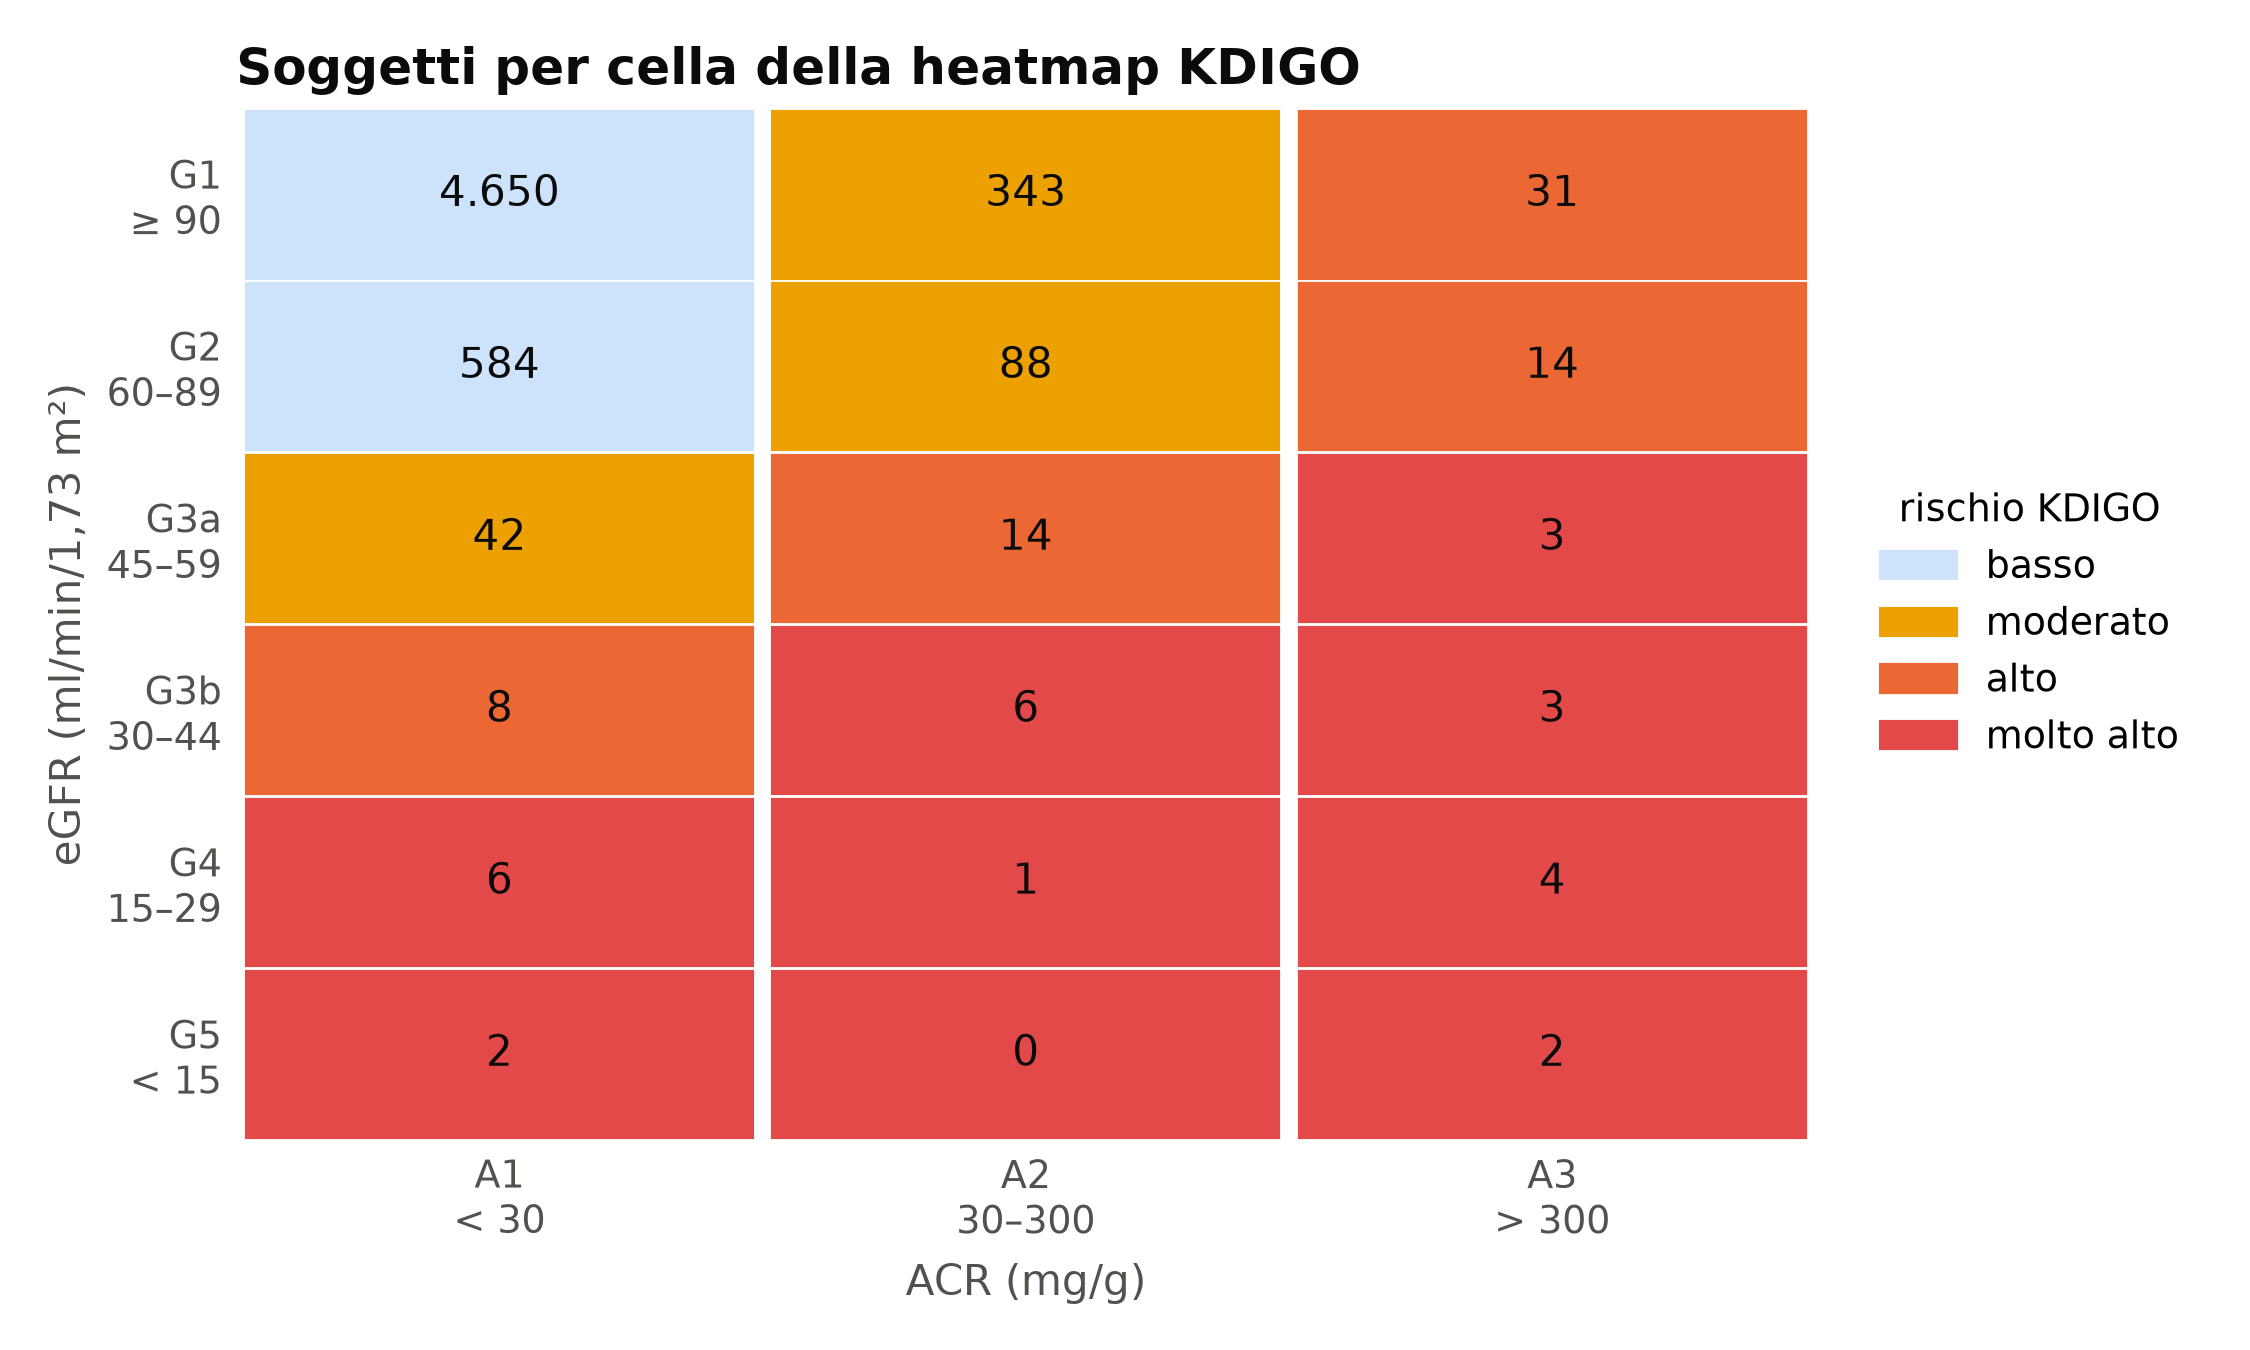
\includegraphics[width=0.75\textwidth]{../analytics/dataset/01_kdigo_heatmap.png}
	\caption{Soggetti eleggibili nelle celle della classificazione KDIGO (categorie di filtrazione G1--G5 per categorie di albuminuria A1--A3), colorate per livello di rischio. La massa dei positivi sta nelle celle G1--G2 con A2: il bersaglio è dominato dall'albuminuria con filtrazione conservata, mentre i livelli alto e molto alto contano insieme 94 soggetti.}
	\label{fig:heatmap}
\end{figure}

\subsection{Criticità dei dati di partenza}

Prima di descrivere la procedura conviene dichiarare i limiti dei dati, perché motivano molte delle scelte.

\begin{enumerate}
	
	\item \textbf{Unità non documentate.} Sulle 4.350 righe del training vale esattamente $\texttt{UMAUCR} = 176{,}8 \cdot \texttt{UmALB}/\texttt{UCRE}$, ma le unità di \texttt{UmALB} e \texttt{UCRE} non sono documentate. Se la creatinina urinaria fosse in mg/dL il fattore corretto sarebbe 100, e la soglia di 30~mg/g corrisponderebbe a $\texttt{UMAUCR} \geq 53{,}04$. L'effetto è misurato con un'analisi di sensibilità.
	
	\item \textbf{Colonna \texttt{GFR} non standard.} I valori presenti nella colonna \texttt{GFR} non sono riconducibili ad alcuna equazione nota (CKD-EPI 2009 e 2021, MDRD, MDRD cinese, Cockcroft-Gault). L'eGFR è quindi ricalcolato mediante CKD-EPI 2021 basata sulla sola creatinina, senza coefficiente etnico~\cite{inker_new_2021,stevens_kdigo_2024}.
	
	\item \textbf{Codice 9 per \enquote{sconosciuto}.} In 26 colonne il dizionario usa 9 come valore mancante.
	
	\item \textbf{Valori mancanti.} Il 38\% dei soggetti del training ha almeno un valore mancante fra le variabili in ingresso.
	
	\item \textbf{Struttura per giornata di raccolta.} la prevalenza dei positivi varia fra il 4,5\% e il 24,5\% nelle 39 giornate. Nelle giornate con creatinina urinaria mediana più bassa la quota di ACR $\geq 30$ cresce, mentre l'albumina urinaria non segue lo stesso andamento (Figura~\ref{fig:ucre-giornata}). La giornata non entra fra i predittori.
	
	\item \textbf{Sbilanciamento e livelli gravi rari.} I positivi sono il 9,77\% e il livello molto alto conta 27 soggetti. Il problema guida la separazione del test e le tecniche di bilanciamento.
\end{enumerate}
	
	\begin{figure}[H]
		\centering
		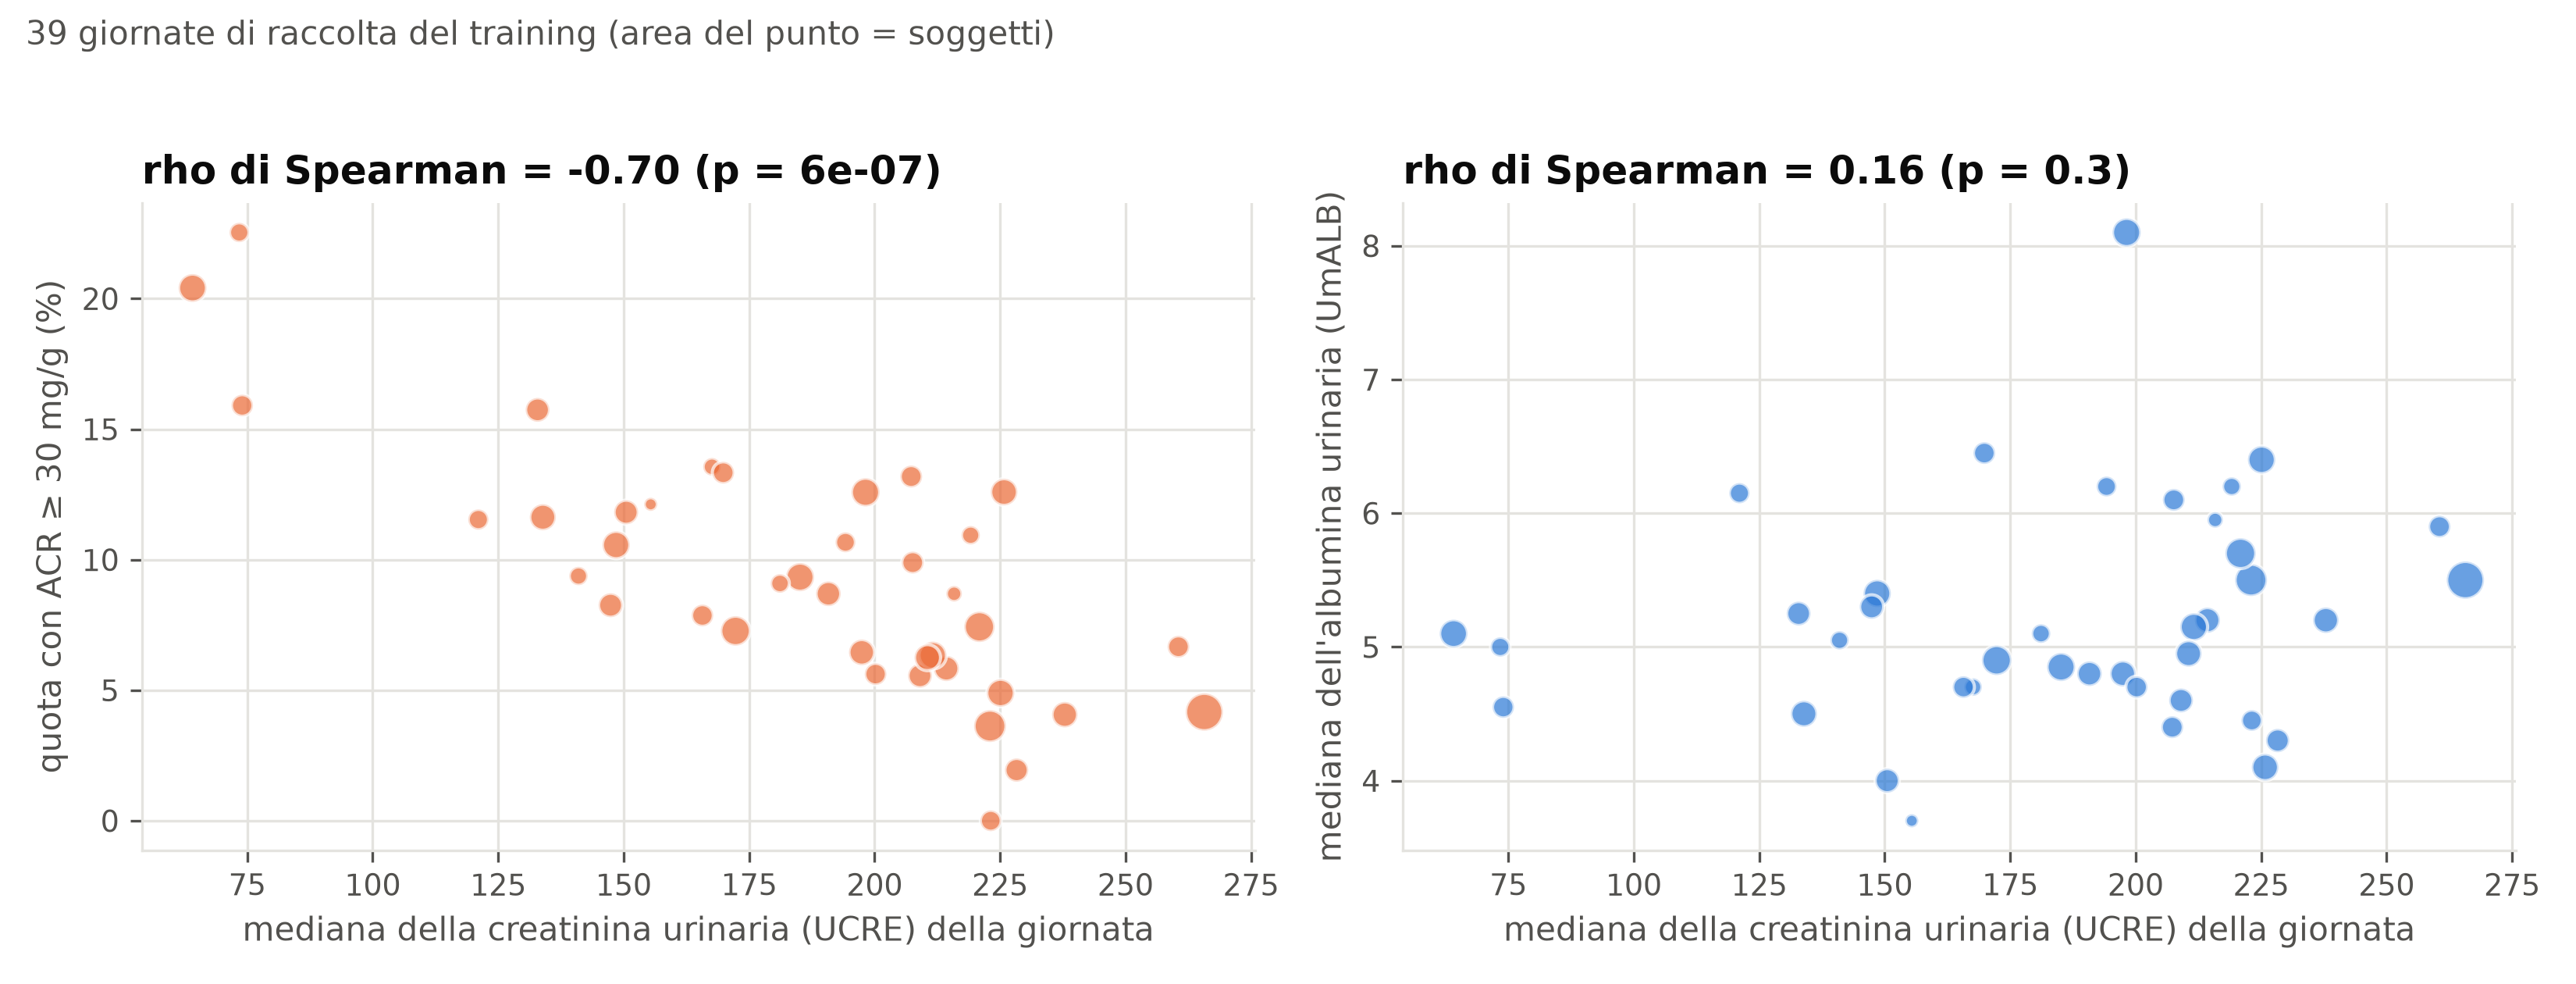
\includegraphics[width=\textwidth]{../analytics/phase_d/03_urine_creatinine_by_day.png}
		\caption{Giornate di raccolta del training (area del punto proporzionale ai soggetti). A sinistra, la quota di soggetti con ACR $\geq 30$ diminuisce al crescere della creatinina urinaria mediana della giornata (rho di Spearman $-0{,}70$); a destra, l'albumina urinaria mediana non mostra la stessa relazione ($+0{,}16$). Parte della variazione dell'ACR fra giornate dipende quindi dal denominatore del rapporto e non dall'albuminuria.}
		\label{fig:ucre-giornata}
	\end{figure}
	
\subsection{Popolazione esterna}

La coorte di sviluppo non consente due verifiche: osservare se il comportamento dei modelli si ripete in una popolazione diversa e collegare il punteggio a un esito successivo alla misura. Per entrambe si usa la \textit{National Health and Nutrition Examination Survey} (NHANES)~\cite{nhanes_cdc,nhanes_cdc_data}, un'indagine trasversale ripetuta che raccoglie esami di laboratorio, misure antropometriche, pressione arteriosa e anamnesi, e i cui partecipanti adulti sono collegati ai registri di morte. Area geografica, struttura d'età e procedure di laboratorio differiscono da quelle della coorte di sviluppo, ed è proprio questa distanza a renderla adatta come banco di prova esterno.

\paragraph{Cicli e file.} Si usano sette cicli biennali consecutivi, dal 2005--2006 (suffisso \texttt{D}) al 2017--2018 (suffisso \texttt{J}). Per ogni ciclo si leggono i dodici file in formato SAS transport della Tabella~\ref{tab:nhanes-file} e il file pubblico di mortalità collegata, aggiornamento 2019, a larghezza fissa: 91 file in tutto. I record si uniscono tramite l'identificativo \texttt{SEQN} a partire dal file demografico. Chi non ha uno degli esami predittori resta nel campione con il valore mancante.

\begin{table}[H]
	\centering
	\small
	\caption{File e variabili NHANES usati per ciascun ciclo.}
	\label{tab:nhanes-file}
	\begin{tabularx}{\textwidth}{@{}l >{\raggedright\arraybackslash}p{5.2cm} >{\raggedright\arraybackslash}X@{}}
		\toprule
		File & Variabili & Contenuto \\
		\midrule
		\texttt{DEMO} & \texttt{RIAGENDR}, \texttt{RIDAGEYR}, \texttt{RIDEXPRG}, \texttt{WTMEC2YR} & sesso, età, gravidanza, peso campionario \\
		\texttt{ALB\_CR} & \texttt{URXUMA}, \texttt{URXUCR}, \texttt{URDACT} & albumina e creatinina urinarie, ACR \\
		\texttt{BIOPRO} & \texttt{LBXSCR}, \texttt{LBXSUA} & creatinina sierica, acido urico \\
		\texttt{CBC} & \texttt{LBXHGB} & emoglobina \\
		\texttt{BMX} & \texttt{BMXBMI}, \texttt{BMXWAIST} & BMI, circonferenza vita \\
		\texttt{BPX} & \texttt{BPXSY1}--\texttt{4}, \texttt{BPXDI1}--\texttt{4} & pressione sistolica e diastolica \\
		\texttt{GHB}, \texttt{GLU} & \texttt{LBXGH}, \texttt{LBXGLU} & HbA1c, glicemia a digiuno \\
		\texttt{TRIGLY}, \texttt{HDL} & \texttt{LBXTR}, \texttt{LBDHDD} & trigliceridi, colesterolo HDL \\
		\texttt{DIQ}, \texttt{BPQ} & \texttt{DIQ010}, \texttt{BPQ020} & diabete e ipertensione diagnosticati, riferiti dal partecipante \\
		mortalità & \texttt{eligstat}, \texttt{mortstat}, \texttt{ucod}, \texttt{permth} & eleggibilità al collegamento, stato in vita, causa principale, mesi di follow-up \\
		\bottomrule
	\end{tabularx}
\end{table}

\paragraph{Criteri di inclusione.} I criteri, fissati nel piano prima dei risultati, si applicano nell'ordine della Tabella~\ref{tab:nhanes-inclusione}. Le numerosità iniziale e finale sono salvate dal codice; quelle intermedie derivano dall'applicazione in sequenza degli stessi filtri.

\begin{table}[H]
	\centering
	\small
	\caption{Selezione del campione NHANES.}
	\label{tab:nhanes-inclusione}
	\begin{tabular}{@{}clr@{}}
		\toprule
		Passo & Criterio & Soggetti \\
		\midrule
		-- & partecipanti dei sette cicli & 70.190 \\
		1 & età $\geq 20$ anni & 39.749 \\
		2 & esclusione della gravidanza (\texttt{RIDEXPRG} $=1$) & 39.041 \\
		3 & eleggibili al collegamento con la mortalità (\texttt{eligstat} $=1$) & 38.924 \\
		4 & albumina, creatinina urinaria e ACR $>0$ & 36.450 \\
		5 & eGFR calcolabile & 34.494 \\
		6 & tempo di follow-up e stato in vita presenti & 34.494 \\
		\bottomrule
	\end{tabular}
\end{table}

\paragraph{Armonizzazione.} Per il ciclo 2005--2006 la creatinina sierica è ricalibrata con la correzione del CDC, $S_{cr}^{\mathrm{cal}} = -0{,}016 + 0{,}978\,S_{cr}$. Nei cicli 2005--2008 il file non contiene l'ACR, che si calcola come $100 \cdot \texttt{URXUMA}/\texttt{URXUCR}$ (mg/g), la stessa formula del CDC. L'eGFR segue l'Equazione~\eqref{eq:ckdepi}, con la creatinina già in mg/dL. Le pressioni sono la media delle letture disponibili (fino a quattro) con valore positivo. L'etichetta segue l'Equazione~\eqref{eq:target} e interessa il 17,6\% del campione.

\paragraph{Pesi campionari.} La domanda riguarda discriminazione e associazione dentro il campione, non la prevalenza nella popolazione statunitense: le analisi principali non sono pesate. Il peso \texttt{WTMEC2YR} entra solo in una sensibilità del modello di Cox, senza riscalarlo sui sette cicli e senza strati né unità primarie di campionamento; per questo la sensibilità è dichiarata non valida. I risultati descrivono il campione, non la popolazione.

\paragraph{Follow-up.} Il tempo di osservazione ha mediana 87 mesi; la chiusura del follow-up è il 31 dicembre 2019. Nel campione si contano 3.590 morti, di cui 1.102 per cause cardiovascolari.

\paragraph{Limiti.} Diabete e ipertensione sono riferiti dal partecipante, mentre nella coorte di sviluppo la variabile \texttt{DM} non coincide con la sola diagnosi nota. L'ACR deriva da una sola misura. Nei file pubblici il NCHS sostituisce alcuni tempi e alcune cause di morte con valori sintetici, per tutela della riservatezza.

\section{Pre-elaborazione e preparazione del dato}

\subsection{Costruzione dell'etichetta}

Il dataset non contiene un'etichetta affidabile della malattia renale, quindi l'etichetta va costruita dagli esami renali secondo la definizione KDIGO~\cite{stevens_kdigo_2024}. Per la filtrazione si usa l'equazione CKD-EPI 2021, priva del coefficiente etnico~\cite{inker_new_2021}:
\begin{equation}
	\mathrm{eGFR} = 142 \cdot \min\!\left(\frac{S_{cr}}{\kappa},1\right)^{\alpha} \cdot \max\!\left(\frac{S_{cr}}{\kappa},1\right)^{-1{,}200} \cdot 0{,}9938^{\,\text{età}} \cdot \delta_F ,
	\label{eq:ckdepi}
\end{equation}
dove $S_{cr}$ è la creatinina sierica in mg/dL (\texttt{SCRE}, in \si{\micro\mole\per\liter}, divisa per 88,4), $\kappa = 0{,}7$ e $\alpha = -0{,}241$ nelle donne, $\kappa = 0{,}9$ e $\alpha = -0{,}302$ negli uomini, e $\delta_F = 1{,}012$ nelle donne e 1 negli uomini. L'etichetta è
\begin{equation}
	y = \mathbf{1}\left[\,\mathrm{ACR} \geq 30 \ \lor \ \mathrm{eGFR} < 60\,\right].
	\label{eq:target}
\end{equation}

Il livello di rischio segue la mappa KDIGO: \emph{basso} per G1--G2 con A1; \emph{moderato} per G1--G2 con A2 e per G3a con A1; \emph{alto} per G1--G2 con A3, G3a con A2 e G3b con A1; \emph{molto alto} in tutte le altre celle. Il livello non è mai un bersaglio di addestramento. Serve per stratificare lo split, valutare i modelli e per pesare o generare esempi in solamente due tecniche di bilanciamento.

Sono state scartate due alternative.
\begin{itemize}
	\item \textbf{La colonna \texttt{DN}}, coincide con la sola concentrazione di albumina urinaria $\geq 30$ (455 casi su 456), ignora la filtrazione e non corrisponde alla definizione KDIGO.
	
	\item \textbf{Il bersaglio a quattro classi}, perché il livello molto alto conta solamente 27 soggetti.
\end{itemize}

\subsection{Separazione dell'insieme di test}

L'insieme di test viene separato prima di qualsiasi stima che impari dai dati. Deve conservare la prevalenza reale e i livelli KDIGO veri dei soggetti, perché su di esso si verificano le conclusioni.

La separazione è un holdout 75/25 stratificato su otto strati (quattro livelli KDIGO per due stati di diabete), con seme 42. La proporzione è stata scelta in base al numero di eventi nel test, che dovrebbe essere almeno 100~\cite{collins_tripodai_2024} (Tabella~\ref{tab:proporzioni}). La proporzione 80/20 lascerebbe nel test 5 casi molto alti e 18 diabetici positivi; la 70/30 toglierebbe al training 28 positivi rispetto a quella scelta.

\begin{table}[H]
	\centering
	\small
	\caption{Numerosità del test per tre proporzioni di split, a parità di seme e stratificazione.}
	\label{tab:proporzioni}
	\begin{tabular}{@{}lrrrrr@{}}
		\toprule
		Split & Test & Positivi test & Positivi training & Molto alto test & Diabetici positivi test \\
		\midrule
		80/20 & 1.161 & 113 & 454 & 5 & 18 \\
		75/25 & 1.451 & 142 & 425 & 6 & 23 \\
		70/30 & 1.741 & 170 & 397 & 8 & 27 \\
		\bottomrule
	\end{tabular}
\end{table}

La stratificazione sul livello KDIGO, e non sul solo bersaglio binario, serve a garantire la presenza dei casi gravi in entrambi gli insiemi. In 1.000 split stratificati sul solo bersaglio, i casi molto alti finiti nel test variano da 1 a 14; in 1.000 split non stratificati, da 0 a 15 (Figura~\ref{fig:stratificazione}). 

\begin{figure}[H]
	\centering
	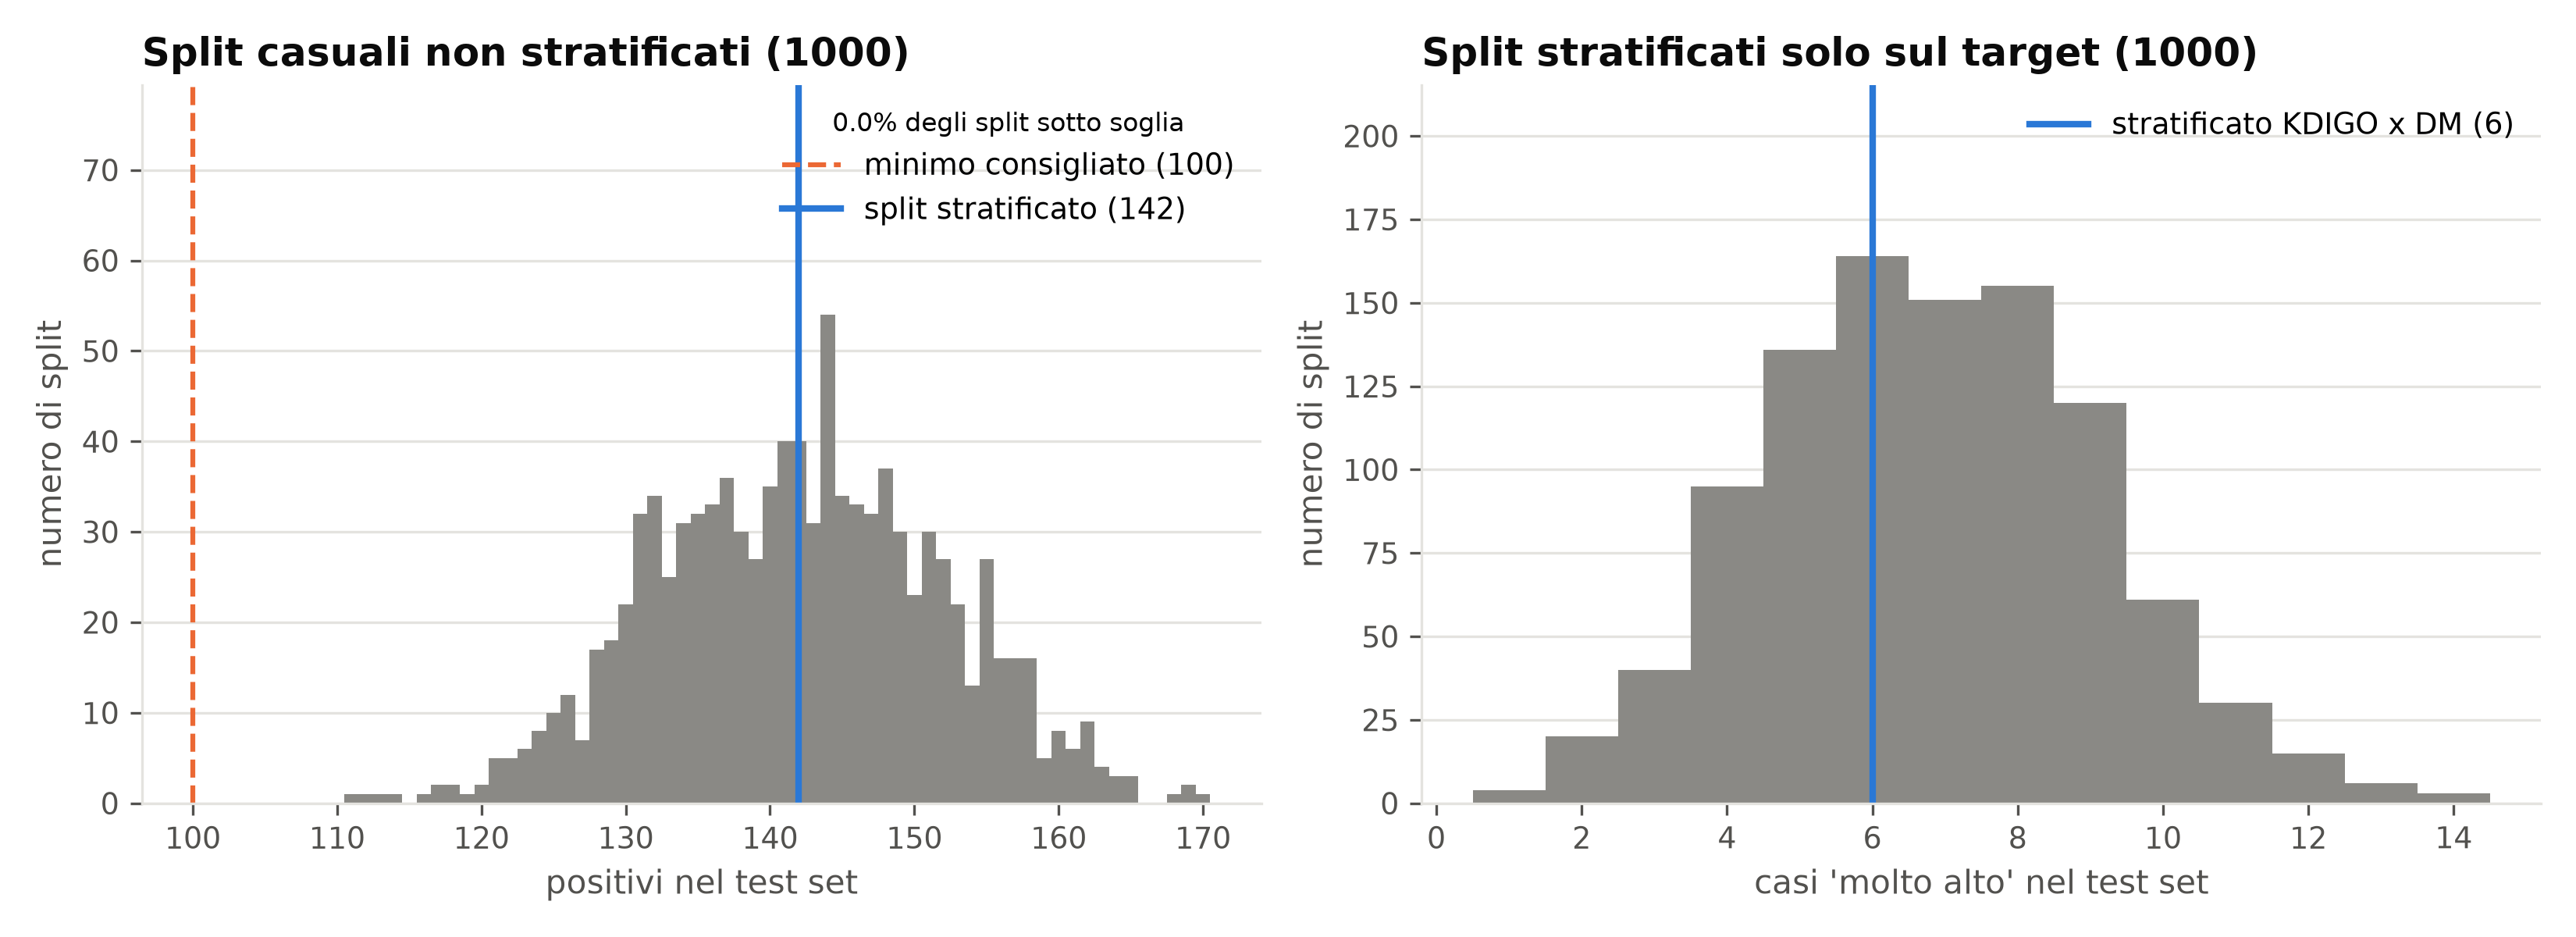
\includegraphics[width=\textwidth]{../analytics/split/04_stratification_simulation.png}
	\caption{Simulazione di 1.000 split 75/25. A sinistra, split non stratificati: il numero di positivi nel test varia ampiamente pur restando sopra la soglia di 100 eventi. A destra, split stratificati sul solo bersaglio: i casi molto alti nel test variano da 1 a 14. Lo split adottato (linea blu) ne contiene sempre 6.}
	\label{fig:stratificazione}
\end{figure}

L'equilibrio fra i due insiemi è verificato con la differenza media standardizzata.

\begin{equation}
	\mathrm{SMD} = \frac{\lvert \bar{x}_{\text{train}} - \bar{x}_{\text{test}} \rvert}{\sqrt{(s^2_{\text{train}} + s^2_{\text{test}})/2}} ,
\end{equation}
su bersaglio, diabete e 15 variabili cliniche. Tutti i valori sono inferiori a 0,1, con un massimo di 0,059 per la pressione sistolica.

Sono state scartate tre alternative. La separazione temporale è priva di significato, perché le 39 giornate coprono circa due mesi. La separazione per giornate intere (validazione \textit{internal-external}) non è stata eseguita ed è dichiarata come limite. La sola validazione incrociata senza test è stata esclusa perché serve un metro fisso e comune a tutte le tecniche. Lo split è stato rifatto dopo l'abbandono di \texttt{DN}: la versione precedente, stratificata su quella colonna, collocava nel test 15 dei 27 casi molto alti. Il file \texttt{test.csv} viene letto soltanto dal rapporto descrittivo dello split e dal modulo di conferma finale.

\subsection{Codifica}

Il codice distingue tre tipi di codifica:
\begin{itemize}
	\item \texttt{HypertenHis}, che nei dati vale soltanto 1 o vuoto: il vuoto è codificato come 0, con 147 \enquote{si} nel training.
	
	\item \texttt{Gender}, da 1/2 a 0 = maschio e 1 = femmina.
	
	\item \texttt{Smoking}, \texttt{Drinking} e \texttt{Tea}, da 1/2/3 a 0/1/2, come variabili ordinali.
\end{itemize}

Nessuna variabile è codificata one-hot, questo tipo di codifica permetterebbe alle tecniche di generazione sintetica di produrre combinazioni impossibili.

\subsection{Standardizzazione e imputazione}

L'analisi dei soli casi completi eliminerebbe il 38\% dei soggetti del training e introdurrebbe distorsione se i dati non mancano completamente a caso. Le variabili con più del 15\% di valori mancanti sono escluse; le altre vengono imputate. Il valore massimo ammesso è del 13,1\%(\texttt{Tea});

La pipeline di pre-processing adotta un'architettura a due stadi stimata rigorosamente all'interno di ciascun fold di addestramento per prevenire qualsiasi forma di leakage. Nel primo stadio le 60 variabili continue sono standardizzate mediante algoritmo \texttt{z-score} con parametri di posizione e scala stimati sui soli casi osservati, mentre le restanti feature categoriche sono state imputate mediante una tecnica di imputazione per moda. Nel secondo stadio, sull'intera matrice a 74 feature è stato applicato l'imputatore iterativo \texttt{MissForest}. Non sono stati inclusi indicatori espliciti di missingness per scongiurare fenomeni di \textit{shortcut learning} e \textit{confounding}, aggiungerne creerebbe una correlazione spuria fra il lotto di campionamento e il target, facendo imparare al modello la giornata di raccolta e non la persona.

Sono stati confrontati quattro candidati, in ordine di complessità crescente:
\begin{itemize}
	\item mediana;
	\item $k$ vicini con $k = 5$
	\item MICE, implementato con \texttt{IterativeImputer} di scikit-learn e regressione bayesiana, 10 iterazioni, una sola imputazione;
	\item una variante di MissForest, implementata con \texttt{IterativeImputer} ed \texttt{ExtraTreesRegressor}: 50 alberi, \texttt{min\_samples\_leaf} = 5, $\sqrt{p}$ variabili per divisione, 5 iterazioni, colonne complete usate solo come predittori.
\end{itemize}

Il confronto valuta i metodi su cinque fold stratificati per livello KDIGO (seme 42) secondo due criteri: l'errore di ricostruzione su un 10\% di dati mascherati (RMSE e MAE standardizzati) e la prestazione predittiva a valle (PR-AUC e AUC di una regressione logica fissa). Poiché le prestazioni a valle risultano indistinguibili, la selezione adotta la regola dell'errore standard~\cite{hastie_elements_2009} applicata all'RMSE, privilegiando la fedeltà di ricostruzione sui dati osservati.

La scelta finale, dopo i confronti, ha visto vincitore il MissForest. La differenza di RMSE fa $k$ vicini e MissForest è $+0{,}060 \pm 0{,}010$, con MissForest migliore in 5 fold su 5, mentre la differenza di PR-AUC ($+0{,}0014 \pm 0{,}0015$) non è significativa. Inoltre una ricostruzione con meno errori aiuta le tecniche di bilanciamento o generazione sintetica nella replica di artefatti fedeli.

\begin{table}[H]
	\centering
	\small
	\caption{Confronto dei metodi di imputazione sull'insieme principale (5 fold sul training, media $\pm$ errore standard). RMSE in unità standardizzate sui valori nascosti; PR-AUC di una regressione logistica fissa addestrata sui dati imputati.}
	\label{tab:imputazione}
	\begin{tabular}{@{}lccccr@{}}
		\toprule
		Metodo & RMSE & MAE & PR-AUC & AUC & Tempo (s) \\
		\midrule
		Mediana & $1{,}038 \pm 0{,}047$ & 0,678 & $0{,}252 \pm 0{,}030$ & 0,693 & 1 \\
		$k$ vicini & $0{,}793 \pm 0{,}057$ & 0,505 & $0{,}259 \pm 0{,}032$ & 0,695 & 11 \\
		MICE & $1{,}252 \pm 0{,}135$ & 0,318 & $0{,}257 \pm 0{,}032$ & 0,697 & 70 \\
		MissForest & $0{,}734 \pm 0{,}066$ & 0,442 & $0{,}257 \pm 0{,}031$ & 0,696 & 305 \\
		\bottomrule
	\end{tabular}
\end{table}

\section{Caratteristiche in ingresso}

Il nucleo di questa fase è la scelta di quali colonne del dataset possano entrare nel modello. Ogni colonna è assegnata in configurazione a esattamente un gruppo per la valutazione, un test automatico impedisce l'ingresso in input al modello di colonne non valutate.

\subsection{Variabili ammesse}

Le variabili ammesse sono 74, di cui 60 numeriche e 14 categoriche (Tabella~\ref{tab:variabili}). Il dizionario del dataset non riporta le unità di misura. Il dizionario del dataset non riporta le unità di misura; la loro conformità agli standard del Sistema Internazionale clinico è stata verificata empiricamente mediante dodici formule fisiologiche note (tra cui \texttt{BMI}, \texttt{HOMA-IR}, \texttt{FIB-4} e indici eritrocitari), tutte coincidenti con i valori attesi (rapporto mediano tra osservato e atteso pari a 1).

\begin{table}[H]
	\centering
	\small
	\caption{Le 74 variabili in ingresso, raggruppate per famiglia (N = numerica, C = categorica o ordinale).}
	\label{tab:variabili}
	\begin{tabularx}{\textwidth}{@{}l >{\raggedright\arraybackslash}X c r@{}}
		\toprule
		Famiglia & Variabili & Tipo & n \\
		\midrule
		Anagrafica & \texttt{Age}, \texttt{Gender} & N, C & 2 \\
		Antropometria e composizione corporea & \texttt{Height}, \texttt{Weight}, \texttt{BMI}, \texttt{waist1}, \texttt{hip}, \texttt{WHR}, \texttt{Fat} & N & 7 \\
		Parametri emodinamici & \texttt{HR}, \texttt{Bpsys}, \texttt{Bpdia} & N & 3 \\
		Metabolismo glucidico e insulinico & \texttt{FPG}, \texttt{PG2h}, \texttt{HbA1c}, \texttt{GA}, \texttt{FINS}, \texttt{INS2h}, \texttt{FCP}, \texttt{CP2h}, \texttt{HomaIR}, \texttt{ISIGutt} & N & 10 \\
		Lipidi & \texttt{CHOL}, \texttt{TG}, \texttt{HDL}, \texttt{LDL} & N & 4 \\
		Funzione epatica e proteine & \texttt{ALT}, \texttt{AST}, \texttt{ASTALT}, \texttt{GGT}, \texttt{ALP}, \texttt{TBIL}, \texttt{DBIL}, \texttt{TP}, \texttt{ALB}, \texttt{AG}, \texttt{FIB4} & N & 11 \\
		Acido urico & \texttt{SUA} & N & 1 \\
		Emocromo & \texttt{WBC}, \texttt{RBC}, \texttt{HGB}, \texttt{HCT}, \texttt{MCV}, \texttt{MCH}, \texttt{MCHC}, \texttt{RDWCV}, \texttt{RDWSD}, \texttt{PLT}, \texttt{MPV}, \texttt{PDW}, \texttt{PCT}, \texttt{NEUT}, \texttt{NEUTcount}, \texttt{LYMPH}, \texttt{LYMPHcount}, \texttt{MONO}, \texttt{MONOcount}, \texttt{EO}, \texttt{EOcount}, \texttt{BASO}, \texttt{BASOcount} & N & 23 \\
		Anamnesi & \texttt{DM}, \texttt{DMhis}, \texttt{DMfamilyHistory}, \texttt{HypertenHis} & C & 4 \\
		Complicanze microvascolari non renali & \texttt{DRyd}, \texttt{cataract}, \texttt{MADPN}, \texttt{TFDPN} & C & 4 \\
		Stili di vita & \texttt{Smoking}, \texttt{Drinking}, \texttt{Tea} & C & 3 \\
		Sierologia & \texttt{HbsAg}, \texttt{HCVAb} & C & 2 \\
		\midrule
		Totale & & & 74 \\
		\bottomrule
	\end{tabularx}
\end{table}

\subsection{Variabili escluse}

Le 116 colonne escluse sono riportate per motivo nella Tabella~\ref{tab:esclusioni} e nella Figura~\ref{fig:mappa-colonne}.

\begin{table}[H]
	\centering
	\small
	\caption{Colonne escluse dall'ingresso, per motivo.}
	\label{tab:esclusioni}
	\begin{tabularx}{\textwidth}{@{}>{\raggedright\arraybackslash}p{3.1cm} r >{\raggedright\arraybackslash}X@{}}
		\toprule
		Motivo & n & Esempi e ragione \\
		\midrule
		Leakage del bersaglio & 16 & \texttt{SCRE}, \texttt{UMAUCR}, \texttt{UmALB}, \texttt{UCRE}, \texttt{GFR}, \texttt{DN} e i flag derivati: il bersaglio è calcolato da queste colonne o ne è una copia (\texttt{EUGFR90UACR01} è il bersaglio calcolato con il \texttt{GFR} originale) \\
		Esami e diagnosi renali & 2 & \texttt{BUN}, \texttt{RF}: violano il principio \enquote{senza esami renali}; \texttt{RF} è la diagnosi già nota \\
		Amministrative & 5 & \texttt{NO}, \texttt{Data}, \texttt{filter}, \texttt{GAnum}, \texttt{GAstudy}: non descrivono il soggetto; \texttt{Data} porterebbe l'effetto della giornata \\
		Non documentate & 3 & \texttt{VAR00001} senza etichetta; \texttt{ALT.1}, che vale $\sqrt{\texttt{ALT}}$ con zeri al posto dei mancanti; \texttt{DF}, con codifica incoerente con il dizionario \\
		Vuote o di sottogruppo & 22 & colonne con oltre il 50\% di mancanti, costanti, o compilate solo da fumatori e bevitori \\
		Questionario di conoscenza & 7 & misurano la conoscenza del diabete, non lo stato di salute \\
		Derivati a soglia & 37 & categorizzazioni di variabili continue già presenti (\texttt{BMI25}, \texttt{Anemia}, \texttt{AgeGroup}, \dots): multicollinearità e soggetti incoerenti nella generazione sintetica \\
		Misure duplicate & 1 & \texttt{Waist2}, seconda misura della vita ($r = 0{,}86$ con \texttt{waist1}) \\
		Combinazioni lineari & 2 & $\texttt{IDBIL} = \texttt{TBIL} - \texttt{DBIL}$; $\texttt{GLO} = \texttt{TP} - \texttt{ALB}$ \\
		Comorbidità con codice 9 & 15 & dopo la ricodifica di 9 come mancante superano il 15\% di mancanti; il composito cardiovascolare ha il 25,4\% di mancanti e prevalenza del bersaglio piatta (10,1\% contro 9,1\%) \\
		Indici instabili & 1 & $\texttt{Homa}\beta = 20 \cdot \texttt{FINS}/(\texttt{FPG} - 3{,}5)$: diverge per glicemie vicine a 3,5 (9 valori oltre 1.000 nel training) \\
		Mancanti oltre il 15\% & 5 & \texttt{leg}, \texttt{LC}, \texttt{LCcount}, \texttt{ALY}, \texttt{ALYcount} \\
		\midrule
		Totale & 116 & \\
		\bottomrule
	\end{tabularx}
\end{table}

\begin{figure}[H]
	\centering
	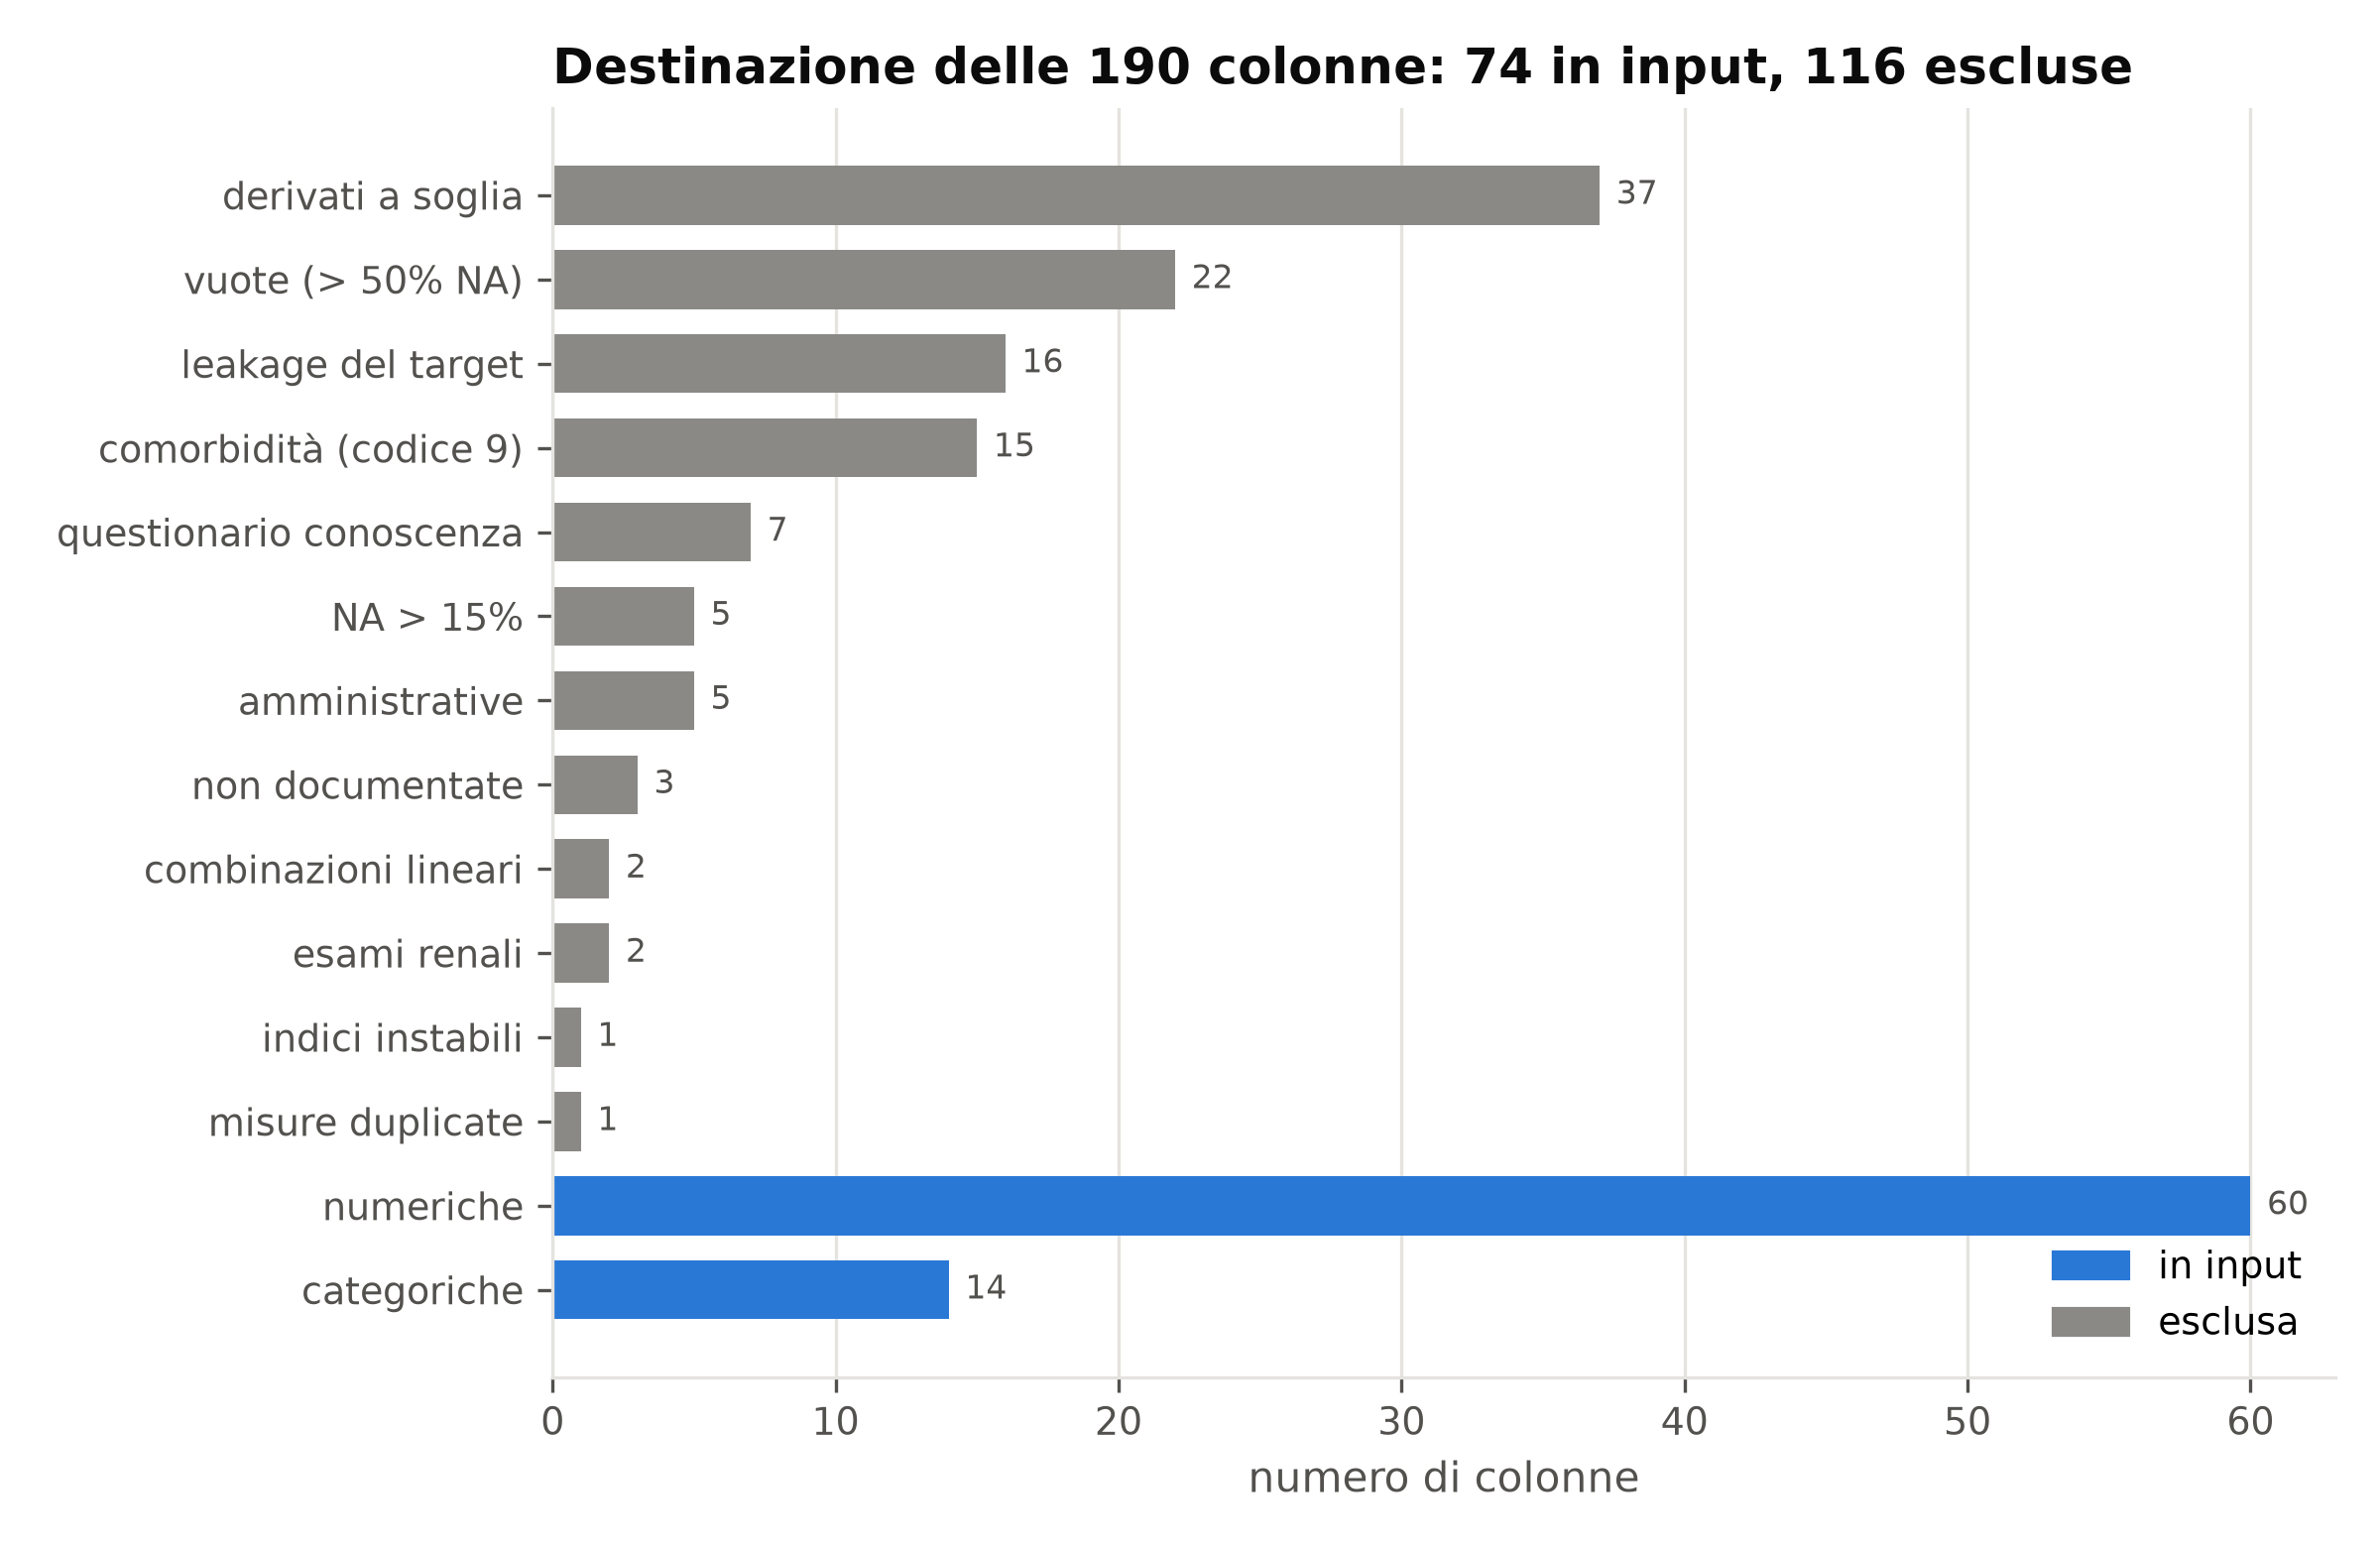
\includegraphics[width=0.85\textwidth]{../analytics/preprocessing/01_column_map.png}
	\caption{Destinazione delle 190 colonne del dataset. Le esclusioni più numerose riguardano i derivati a soglia e le colonne vuote, che non portano informazione nuova; quelle per leakage sono 16 e comprendono tutte le grandezze da cui è calcolato il bersaglio.}
	\label{fig:mappa-colonne}
\end{figure}

Sono stati invece tenuti gli indici clinici continui non lineari, che non si ricavano con una somma dalle altre colonne: \texttt{BMI}, \texttt{WHR}, \texttt{HomaIR}, \texttt{ISIGutt}, \texttt{FIB4} e \texttt{ASTALT}.

\subsection{Controllo del leakage residuo}

Escludere le colonne note non basta: un predittore non renale potrebbe trasportare il bersaglio in modo indiretto. Sono state quindi previste due difese. La prima è un'asserzione nel codice: la selezione si interrompe se fra le variabili compare una colonna di leakage, un esame renale o una colonna con codice 9. La seconda è il calcolo, sul solo training, dell'AUC univariata di ogni variabile rispetto al bersaglio, con soglia di allarme a 0,75. Il valore massimo è 0,653 (\texttt{Age}), seguito da \texttt{ALP} (0,631), \texttt{FIB4} (0,623) e \texttt{Bpsys} (0,610) (Figura~\ref{fig:auc-univariata}).

\begin{figure}[H]
	\centering
	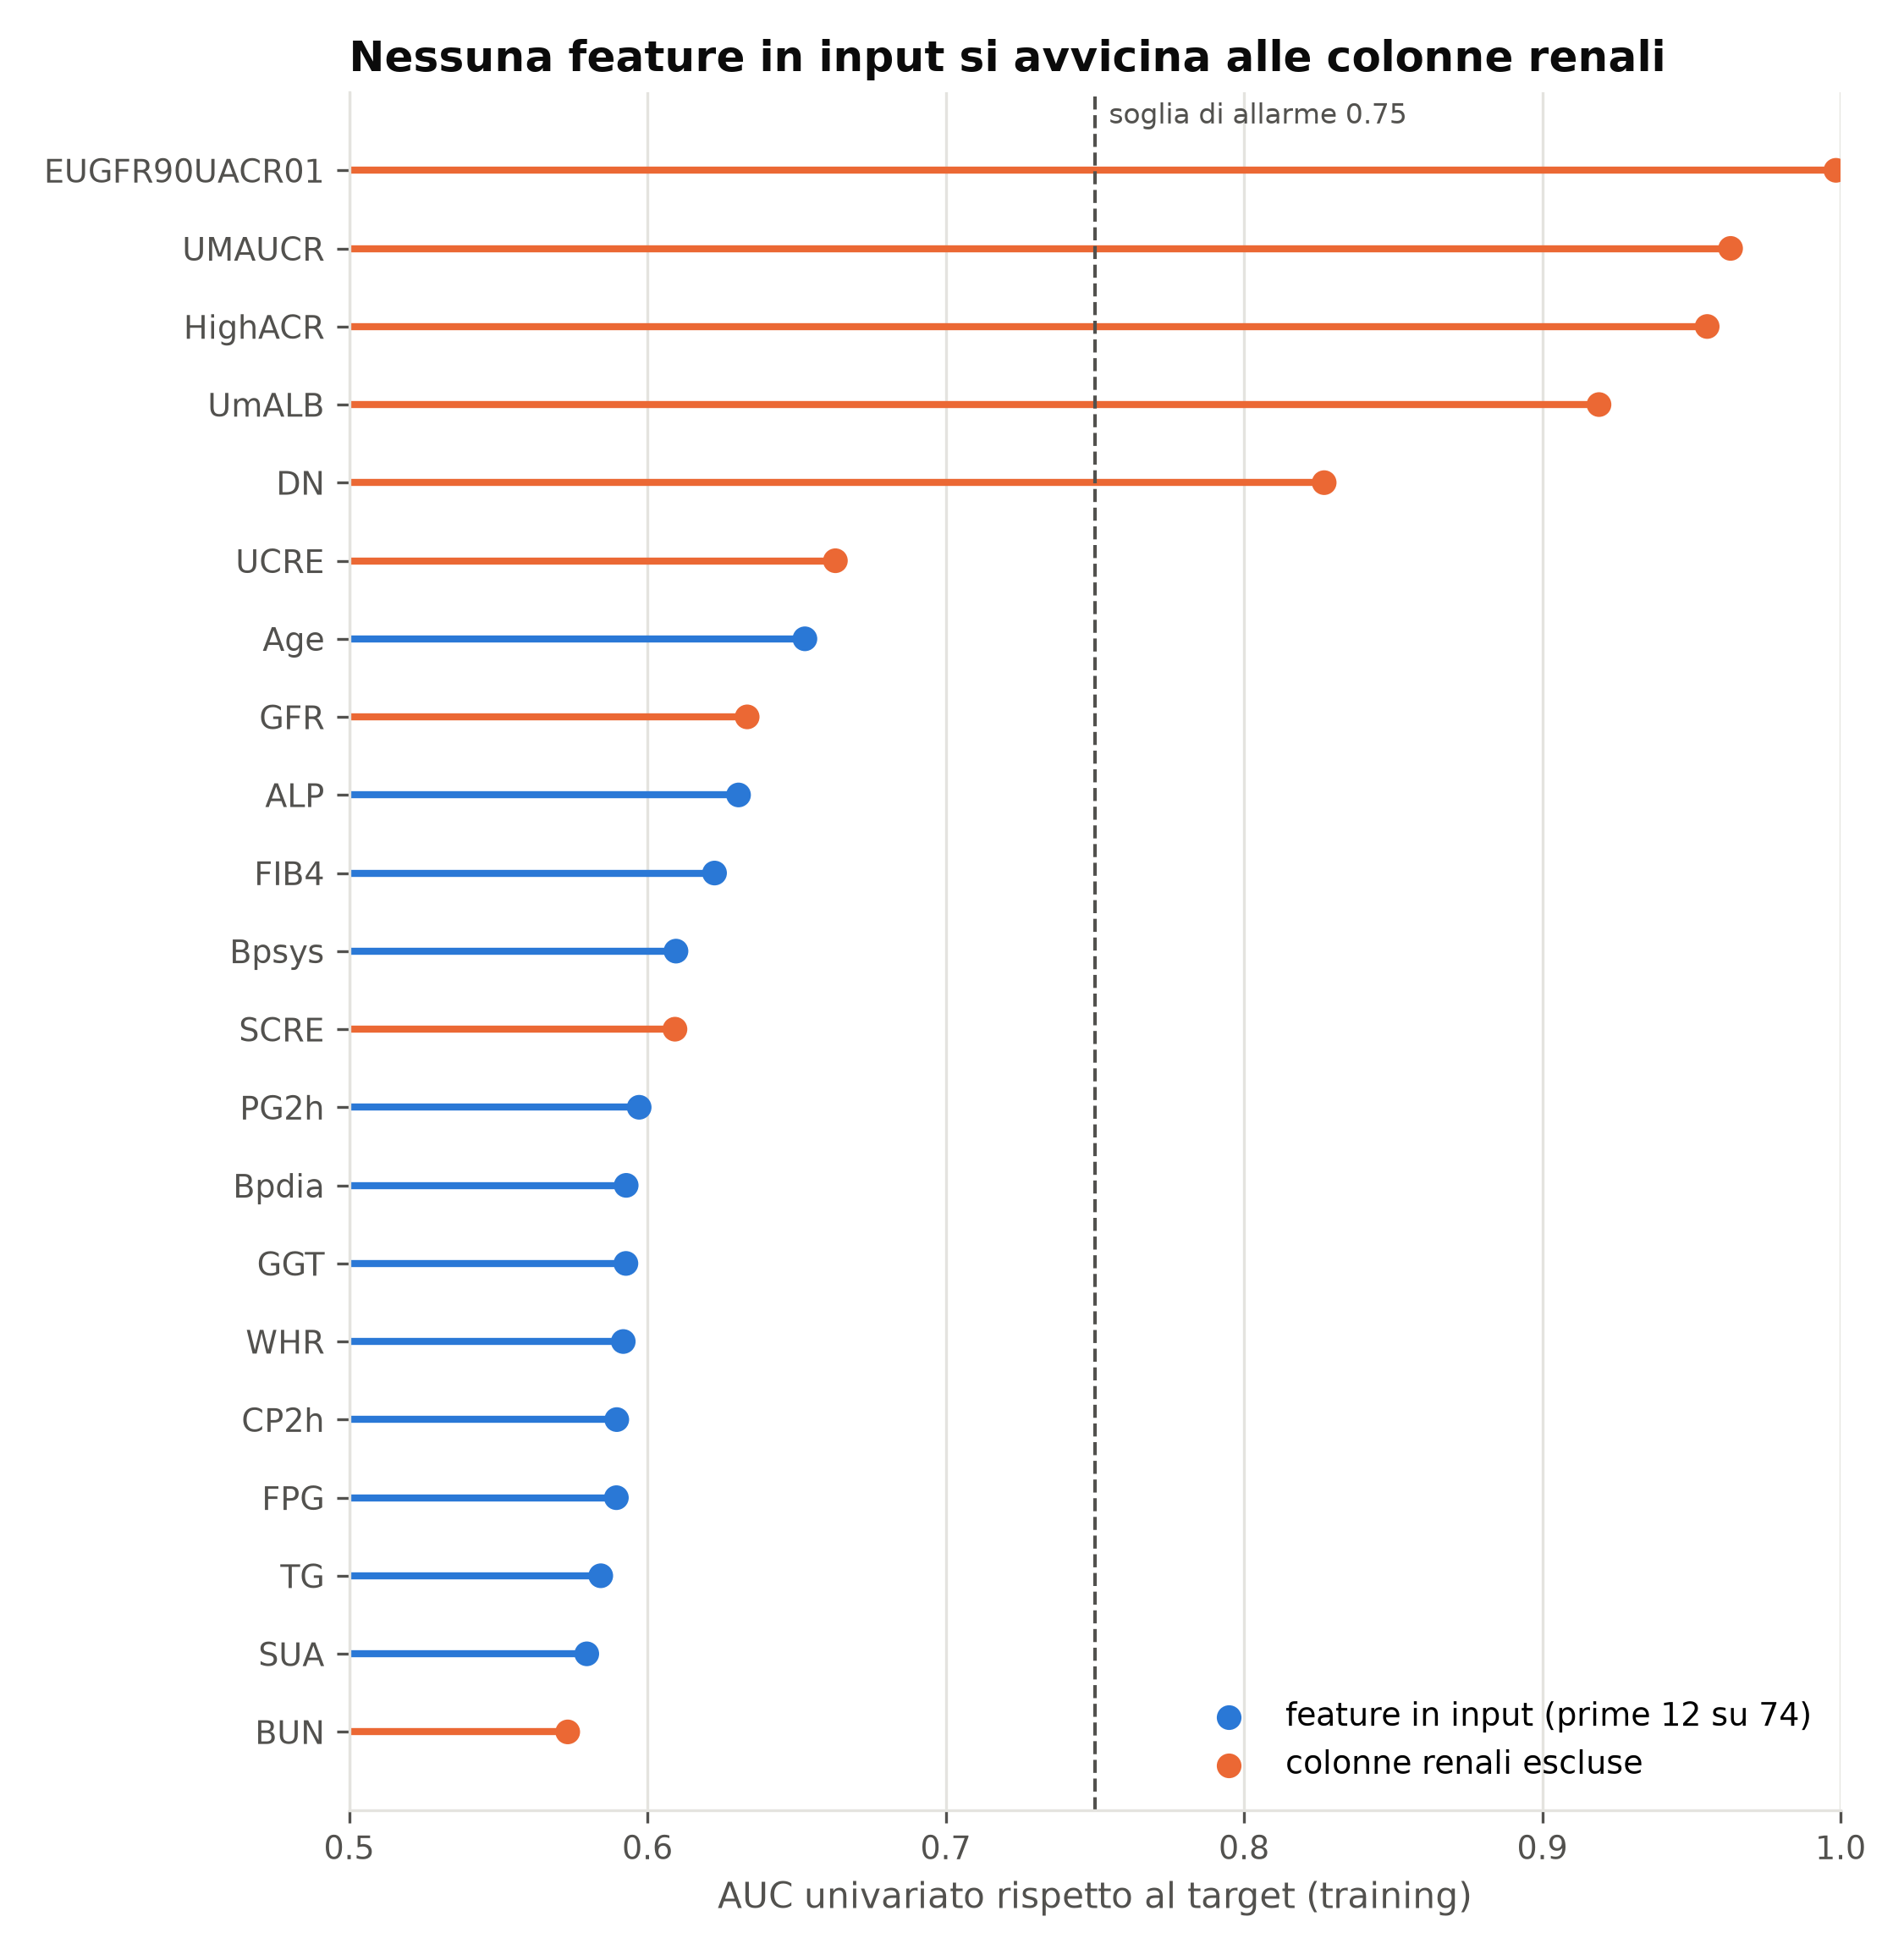
\includegraphics[width=0.7\textwidth]{../analytics/preprocessing/02_univariate_auc.png}
	\caption{AUC univariata sul training delle prime 12 variabili in ingresso (blu) e delle colonne renali escluse (arancione). Le colonne da cui è calcolato il bersaglio si avvicinano a 1, mentre nessuna variabile in ingresso supera la soglia di allarme di 0,75.}
	\label{fig:auc-univariata}
\end{figure}

\subsection{Variabili conseguenza}

Sette variabili ammesse possono essere alterate dalla malattia renale stessa e agire quindi come suoi effetti: \texttt{HGB}, \texttt{RBC} e \texttt{HCT} (anemia), \texttt{SUA} (ridotta escrezione), \texttt{ALB}, \texttt{TP} e \texttt{GA}. Non sono leaker di definzione e restano nell'insieme principale. Per verificare che le prestazioni non dipendano da loro si usa l'insieme di sensibilità \texttt{no\_consequence}, che le esclude e conta quindi 67 variabili.

\section{Modelli e ottimizzazione}

\subsection{Modelli}

I modelli sono stati scelti per famiglia e per ruolo, in ordine di complessità crescente. (Tabella~\ref{tab:modelli}).

\begin{table}[H]
	\centering
	\small
	\caption{Modelli delle fasi confermative.}
	\label{tab:modelli}
	\begin{tabularx}{\textwidth}{@{}>{\raggedright\arraybackslash}p{3cm} >{\raggedright\arraybackslash}X >{\raggedright\arraybackslash}p{3.6cm}@{}}
		\toprule
		Modello & Ruolo & Implementazione \\
		\midrule
		Classificatore di maggioranza & soglia minima e controllo di coerenza: AUC 0,5 e PR-AUC pari alla prevalenza & \texttt{DummyClassifier}, strategia \texttt{prior} \\
		Logistica SCORED & punteggio clinico con i predittori di SCORED~\cite{bang_screening_2007} disponibili: \texttt{Age}, \texttt{Gender}, \texttt{HGB}, \texttt{Bpsys}, \texttt{DM}; coefficienti ristimati & \texttt{LogisticRegression}, nessuna penalizzazione \\
		Logistica penalizzata & modello lineare di riferimento sulle 74 variabili & \texttt{LogisticRegression}, solver \texttt{saga}, elastic net \\
		Random Forest & insieme di alberi per bagging~\cite{breiman_random_2001} & \texttt{RandomForestClassifier} \\
		XGBoost & insieme di alberi per gradient boosting~\cite{chen_xgboost_2016} & \texttt{XGBClassifier}, \texttt{tree\_method=hist} \\
		\bottomrule
	\end{tabularx}
\end{table}

Ogni modello ha un ruolo preciso.
\begin{itemize}
	\item \textbf{Logistica SCORED.} SCORED è stato scelto perché è il punteggio per la malattia renale occulta più validato esternamente~\cite{echouffo-tcheugui_risk_2012}. Rispetto all'originale, l'età è continua, l'emoglobina sostituisce il flag di anemia e la pressione sistolica misurata sostituisce l'ananmesi di ipertensione. Malattia cardiovascolare, scompenso, arteriopatia periferica e proteinuria non sono disponibili. Con circa 85 eventi per variabile (425/5) non serve penalizzazione.
	
	\item \textbf{Logistica penalizzata.} Con 74 variabili gli eventi per variabile scendono a circa 5,7 (circa 4,6 nei fold di training), sotto la soglia convenzionale di 10~\cite{collins_tripodai_2024}: da qui la penalizzazione. Nei confronti a basso rischio di distorsione la regressione logistica non è inferiore al machine learning~\cite{christodoulou_systematic_2019}.
	
	\item \textbf{Random Forest e xGBoost.} Sono due insiemi di alberi, uno per famiglia, e misurano il contributo delle relazioni non lineari e delle interazioni.
\end{itemize}

Nelle fasi confermative sono stati esclusi LightGBM e CatBoost, ripresi poi nell'analisi esplorativa successiva insieme ad altri come $k$ vicini, SVM, reti neurali e modelli tabellari.

\subsection{Ottimizzazione degli iperparametri}

Gli iperparametri sono scelti con Optuna, campionatore TPE con seme 32 e interruzione anticipata \texttt{MedianPruner}. L'obiettivo è la PR-AUC media (\textit{average precision}) sui 5 fold interni di ciascun fold esterno; dopo ogni fold interno il valore parziale viene comunicato all'interruttore. il budget è di 100 tentativi per modello e per fold esterno, uguale per tutti i modelli e fissato prima dei risultati; gli spazi sono riportati nella tabella~\ref{tab:spazi}.

Il modello finale vincitore dei round di ottimizzazione ripete la ricerca usando i 5 fold esterni come validazione incrociata dell'intero training, e viene poi riaddestrato su tutti i 4.350 soggetti. L'insieme \texttt{no\_consequence} non è ottimizzato: riusa gli iperparametri dell'insieme principale fold per fold, così che l'analisi di sensibilità cambi soltanto le variabili.

\begin{table}[H]
	\centering
	\small
	\caption{Spazi di ricerca degli iperparametri (scala logaritmica dove indicato). Il classificatore di maggioranza e la logistica SCORED non hanno iperparametri.}
	\label{tab:spazi}
	\begin{tabularx}{\textwidth}{@{}l l >{\raggedright\arraybackslash}X@{}}
		\toprule
		Modello & Iperparametro & Intervallo \\
		\midrule
		Logistica penalizzata & \texttt{C} & $10^{-4}$--10 (log) \\
		& \texttt{l1\_ratio} & 0--1 (0 = L2, 1 = L1) \\
		\midrule
		Random Forest & \texttt{n\_estimators} & 100--1000 \\
		& \texttt{max\_depth} & 3--25 \\
		& \texttt{min\_samples\_split} & 2--50 \\
		& \texttt{min\_samples\_leaf} & 1--20 \\
		& \texttt{max\_features} & sqrt, log2, 0,25, 0,5, 0,75 \\
		& \texttt{criterion} & gini, entropy \\
		\midrule
		XGBoost & \texttt{n\_estimators} & 200--1200 \\
		& \texttt{learning\_rate} & 0,01--0,3 (log) \\
		& \texttt{max\_depth} & 3--12 (1--12 nell'analisi di sensibilità e nel bilanciamento) \\
		& \texttt{subsample} & 0,6--1,0 \\
		& \texttt{colsample\_bytree} & 0,5--1,0 \\
		& \texttt{reg\_alpha}, \texttt{reg\_lambda} & 0--5 \\
		\bottomrule
	\end{tabularx}
\end{table}

\subsection{Soglia e fasce di rischio}

Dalla probabilità stimata dal modello derivano una classe e una fascia di rischio. In uno screening un falso negativo è un caso mancato, mentre un falso positivo è un esame in più. La soglia che determina il target dalla probabilità ha, quindi, un compito molto importante. Si sceglie la soglia più alta con sensibilità almeno pari a 0,90 sulle previsioni out-of-fold:
\begin{equation}
	t^{*} = s_{(k)}, \qquad k = \lceil 0{,}90 \cdot n_{+} \rceil ,
\end{equation}
dove $s_{(1)} \geq s_{(2)} \geq \dots$ sono le probabilità dei positivi in ordine decrescente; un soggetto è positivo se $p \geq t^{*}$. La soglia di Youden è scartata perché assume costi uguali per i due errori. Le sensibilità 0,80, 0,85 e 0,95 sono riportate come punti operativi descrittivi.

Le fasce sono quattro, ricavate dai quantili delle probabilità con le stesse proporzioni dei livelli KDIGO nel training (90,2\%, 8,1\%, 1,1\% e 0,5\%); un valore pari al limite va nella fascia superiore. Soglia e fasce dipendono solo dall'ordinamento delle previsioni: restano quindi confrontabili quando il bilanciamento sposta le probabilità. Una volta stimate in validazione incrociata vengono congelate, e non sono mai ristimate sul test o sui sottogruppi.

\subsection{Trattamento dello sbilanciamento}

Con il 9,77\% di positivi la letteratura suggerisce spesso di riequilibrare le classi, ma con modelli forti il riequilibrio non migliora la discriminazione e peggiora la calibrazione~\cite{van_den_goorbergh_harm_2022}. La domanda è quindi se il bilanciamento faccia riconoscere più casi gravi. Sono confrontate sei tecniche principali e due esplorative (Tabella~\ref{tab:bilanciamento}).

\begin{table}[H]
	\centering
	\small
	\caption{Tecniche di bilanciamento. Il rapporto finale fra positivi e negativi delle tecniche di campionamento è 1:1.}
	\label{tab:bilanciamento}
	\begin{tabularx}{\textwidth}{@{}>{\raggedright\arraybackslash}p{3.3cm} >{\raggedright\arraybackslash}X@{}}
		\toprule
		Tecnica & Definizione \\
		\midrule
		Pesi di classe & $w_i = n / (2\, n_{y_i})$: le due classi pesano uguale, media dei pesi 1 \\
		Pesi per livello KDIGO & fra i positivi peso proporzionale al costo del livello (moderato 1, alto 2, molto alto 3), poi riscalato perché positivi e negativi pesino $n/2$ ciascuno \\
		Sottocampionamento & rimozione casuale di negativi fino a 1:1 \\
		Sovracampionamento & duplicazione casuale di positivi fino a 1:1 \\
		SMOTE-NC & interpolazione fra vicini con $k = 5$~\cite{chawla_smote_2002}; le 14 categoriche trattate come nominali \\
		SMOTE-NC per livello & generazione dentro ciascun livello positivo, $k = \min(5, n_\ell - 1)$, quote proporzionali alle numerosità con il metodo del resto più grande \\
		CTGAN (esplorativa) & rete generativa condizionata sulla classe~\cite{xu_modeling_2019}, 300 epoche, lotti da 500, addestrata sull'intero training del fold \\
		CTGAN per livello (esplorativa) & come sopra, condizionata sul livello KDIGO \\
		\bottomrule
	\end{tabularx}
\end{table}

Ogni tecnica è applicata solo alla parte di addestramento di ciascun fold, interno ed esterno, e del training intero; la validazione resta sempre composta da soggetti reali. Il livello KDIGO serve solo per i pesi e la generazione non entra mai fra le variabili. I dati sintetici sono generati una volta per tecnica e per fold, con seme $42 +100\,o + (i + 14)$ per il fold interno e $i$ del fold esterno $o$ (con $o = 5$ e $i$ assente per il training intero), e salvati con un'impronta di controllo. Tutti i modelli vedono così gli stessi dati.

L'ottimizzazione usa 30 tentativi per fold, e il primo tentativo è l'ottimo della fase senza bilanciamento per lo stesso fold. Il budget è motivato dai registri della fase precedente: a 30 tentativi la PR-AUC interna dista in mediana fra 0,0004 e 0,005 dal valore a 100, meno della variabilità fra i fold. 

Poiché il bilanciamento distorce le probabilità~\cite{dal_pozzolo_calibrating_2015,van_den_goorbergh_harm_2022}, si applica una ricalibrazione di Platt annidata~\cite{platt_probabilities_2000}:

\begin{equation}
	p' = \sigma\!\left(a + b \cdot \operatorname{logit}(\tilde p)\right), \qquad \tilde p = \min\!\left(\max(p, 10^{-6}),\, 1 - 10^{-6}\right),
\end{equation}
con $a$ e $b$ stimati sulle previsioni delle righe interne \emph{reali} del fold, prodotte dal modello addestrato sui dati bilanciati. Con pochi eventi Platt è preferibile alla regressione isotonica ~\cite{niculescu-mizil_predicting_2005}. Le probabilità ricalibrate servono per la calibrazione e per le probabilità medie per livello. L'esito primario e le metriche di ordinamento restano sulle probabilità grezze.

\subsection{Modelli esplorativi}

Dopo le prime fasi sopracitate, una serie di analisi esplorative ha cercato di stabilire se si potesse ottenere una discriminazione migliore. La regola di decisione è stata fissata prima dei calcoli. Un candidato migliora se, contro il riferimento con AUROC media sui fold più alta, soddisfa tre condizioni:
\begin{itemize}
	\item differenza di AUROC $\geq 0{,}01$;
	\item limite inferiore dell'intervallo al 95\% maggiore di zero;
	\item p di Holm $< 0{,}05$ fra i candidati.
\end{itemize}
I candidati sono riassunti nella Tabella~\ref{tab:esplorativi}.

\begin{table}[H]
	\centering
	\small
	\caption{Modelli esplorativi. Salvo diversa indicazione: stessi fold, Optuna con TPE e \texttt{MedianPruner}, 30 tentativi, PR-AUC sui fold interni.}
	\label{tab:esplorativi}
	\begin{tabularx}{\textwidth}{@{}>{\raggedright\arraybackslash}p{3.6cm} >{\raggedright\arraybackslash}X@{}}
		\toprule
		Candidato & Descrizione \\
		\midrule
		Media dei riferimenti & media delle probabilità out-of-fold di logistica penalizzata, Random Forest e XGBoost \\
		XGBoost con mancanti nativi & dati non imputati e non scalati \\
		XGBoost con spazio allargato & in più \texttt{min\_child\_weight} 1--50 (log) e \texttt{gamma} 0--5; 100 tentativi \\
		XGBoost senza interruzione & spazio della sezione bilanciamento senza \texttt{MedianPruner} \\
		Logistica tutta standardizzata & anche le categoriche standardizzate \\
		Bersaglio scomposto & un XGBoost per l'albuminuria e uno per eGFR $<60$; $p = 1 - (1-p_A)(1-p_G)$ \\
		CatBoost & \texttt{iterations} 200--1200, \texttt{learning\_rate} 0,01--0,3, \texttt{depth} 1--8, \texttt{l2\_leaf\_reg} 1--10 \\
		LightGBM & \texttt{n\_estimators} 100--1200, \texttt{num\_leaves} 2--64, \texttt{min\_child\_samples} 5--100, campionamenti e regolarizzazioni come XGBoost \\
		EBM & iperparametri predefiniti \\
		TabPFN v2 & nessuna ottimizzazione, esecuzione su CPU \\
		Tri-ensemble su 21 variabili & media dei tre riferimenti addestrati sulle prime 21 variabili, scelte \emph{dentro} ogni fold per rango medio di coefficienti e SHAP \\
		Bersaglio continuo & \texttt{XGBRegressor} su $\log(\texttt{UMAUCR})$; probabilità per ACR $\geq 30$ con logistica sulla stima, stimata sulle previsioni interne \\
		Undici famiglie nuove & Extra Trees, gradient boosting a istogrammi, SVM a kernel RBF, $k$ vicini, Naive Bayes, analisi discriminante lineare e quadratica, MLP, AdaBoost, logistica su spline (GAM), logistica con tutte le interazioni a coppie \\
		ACR e creatinina continui & regressori su $\log(\texttt{UMAUCR})$ e $\log(\texttt{SCRE})$; la soglia entra solo nel calcolo finale della probabilità (Equazione~\ref{eq:combinato}) \\
		Margine KDIGO & un solo bersaglio continuo, la distanza dalla soglia in larghezze di categoria \\
		Stacking e media dei ranghi & meta-modello logistico L2 sulle previsioni out-of-fold di tutti i modelli; media dei ranghi senza parametri \\
		\bottomrule
	\end{tabularx}
\end{table}

Nei modelli senza soglia la condizione eGFR $< 60$ è riscritta come $S_{cr} > S_{60}(\text{età}, \text{sesso})$, la creatinina a cui l'Equazione~\eqref{eq:ckdepi} vale 60. Nel ramo $S_{cr}/\kappa \geq 1$ l'equazione si inverte in forma chiusa:
\begin{equation}
	S_{60} = \kappa \left( \frac{142 \cdot 0{,}9938^{\,\text{età}} \cdot \delta_F}{60} \right)^{1/1{,}2} .
\end{equation}
Dette $\mu_A(x)$ e $\mu_C(x)$ le stime dei due regressori ed $(e_{A,i}, e_{C,i})_{i=1}^{m}$ le coppie di residui out-of-fold interni, la probabilità del bersaglio composito si ottiene dalla distribuzione empirica congiunta dei residui, senza ipotesi di normalità né di indipendenza:
\begin{equation}
	p(x) = 1 - \frac{1}{m} \sum_{i=1}^{m} \mathds{1}\!\left[\mu_A(x) + e_{A,i} < \log 30 \ \land\ \mu_C(x) + e_{C,i} < \log S_{60}(x)\right].
	\label{eq:combinato}
\end{equation}
Sono state provate tre varianti: un LightGBM per bersaglio; la stessa coppia con residui riscalati da un modello della varianza per soggetto (LightGBM su $\log e^2$ con 200 alberi, learning rate 0,05, 7 foglie, almeno 100 campioni per foglia); una rete neurale con due uscite e strati condivisi. Il margine KDIGO è
\begin{equation}
	M = \max\!\left( \frac{\log \mathrm{ACR} - \log 30}{\log 10},\ \frac{\log S_{cr} - \log S_{60}}{\log(60/45)/1{,}2} \right),
\end{equation}
positivo se e solo se $y = 1$. Le due unità di misura sono la larghezza della categoria A2 e quella di G3a.

Lo stacking usa il \textit{cross-fitting}: il meta-modello del fold $k$ è stimato sulle previsioni e sulle etichette degli altri quattro fold, con \texttt{C} scelto per PR-AUC in una validazione a 5 fold su quelle righe. Ricalibrazione e soglie seguono la stessa logica. La prima valutazione ha mostrato che alcuni modelli producono punteggi su scale diverse fra fold (gradient boosting a istogrammi: AUROC aggregata 0,620 contro 0,695 di media dei fold). Si è quindi deciso, dopo averla vista, di trasformare ogni punteggio nel suo percentile dentro il proprio fold esterno, $r/(n+1)$, prima di ricalibrazione, stacking e media dei ranghi. La correzione è dichiarata; i confronti con il riferimento non cambiano, perché usano le AUROC dei singoli fold.

\subsection{Modelli non supervisionati}

Per verificare che cosa emerga dai dati senza l'etichetta e senza le soglie KDIGO sono stati addestrati due metodi non supervisionati: $k$-means~\cite{lloyd_least_1982} e un autoencoder~\cite{hinton_reducing_2006}. Sono stati applicati a insiemi di variabili con e senza esami renali, e da ciascun modello si ricava un punteggio continuo, confrontato solo a posteriori con la definizione KDIGO e con la sola età. L'etichetta non entra mai nell'addestramento. Gli impieghi sono due e dichiarano ciascuno il proprio tipo. Anche qui il dataset input è stato diviso in vari split rappresentati nella Tabella~\ref{tab:insiemi-nonsup}.

\begin{table}[H]
	\centering
	\small
	\caption{Insiemi di variabili delle analisi non supervisionate.}
	\label{tab:insiemi-nonsup}
	\begin{tabularx}{\textwidth}{@{}l >{\raggedright\arraybackslash}X r l@{}}
		\toprule
		Insieme & Colonne & $p$ & Tipo \\
		\midrule
		Split G & le 74 ammesse più \texttt{SCRE}, \texttt{UmALB}, \texttt{UCRE}, \texttt{BUN} grezze & 78 & esplicativo \\
		Split T & tutte le colonne del file, esclusa \texttt{CDSMS} (vuota) & 189 & esplicativo; contiene il bersaglio già calcolato \\
		Ammesse & le 74 della Tabella~\ref{tab:variabili} & 74 & predittivo \\
		Comuni & le 14 della Tabella~\ref{tab:variabili-comuni} & 14 & predittivo, trasportato su NHANES \\
		\bottomrule
	\end{tabularx}
\end{table}


\paragraph{Dati e preelaborazione.} L'analisi predittiva usa i 4.350 soggetti del training e gli stessi 5 fold esterni della Random Forest dell'insieme principale. Dentro ogni fold i mancanti sono sostituiti con la mediana e le colonne standardizzate con media e deviazione standard del fold di addestramento; un'ipertensione non compilata vale 0. Negli split G e T si applicano, dentro il fold: $\log(1+x)$ alle continue con asimmetria superiore a 1 (dopo uno spostamento se compaiono valori non positivi), standardizzazione delle numeriche, moda per le categoriche, MissForest con la configurazione della sezione imputazione, standardizzazione finale ed eliminazione delle colonne a varianza nulla; la validazione è $5 \times 1$ sui fold esterni. Per il trasporto su NHANES il $k$-means è stimato una sola volta sui 4.350 soggetti del training, e mediane e standardizzazione della coorte di sviluppo sono applicate a NHANES.

\paragraph{Limiti.} Il punteggio misura l'atipicità rispetto al gruppo più numeroso, non la malattia. Il numero di gruppi è fissato, non ottimizzato. Lo split T contiene il bersaglio già calcolato e ha valore solo esplicativo.


\chapter{Risultati ottenuti}

\chapter{Conclusioni e sviluppi futuri}

\chapter*{Ringraziamenti}
\addcontentsline{toc}{chapter}{Ringraziamenti}
\clearpage
\cleardoublepage
\addcontentsline{toc}{chapter}{Bibliografia}
\bibliographystyle{unsrt} 
\bibliography{bib}       
\clearpage
\listoffigures
\addcontentsline{toc}{chapter}{\listfigurename}
\clearpage
\listoftables
\addcontentsline{toc}{chapter}{\listtablename}
\clearpage
\end{document}

